\documentclass{article}
\usepackage{graphicx}
\usepackage{xcolor}
\usepackage[margin=3cm]{geometry} % margins might need to change in the future check with professor adam 
\setlength{\parindent}{0pt}
\usepackage{pgfgantt}
\usepackage{booktabs}
\usepackage{graphicx}
\usepackage{float}
\usepackage{times}
\usepackage{fancyhdr,graphicx,amsmath,amssymb}
\usepackage[ruled,vlined]{algorithm2e}
\include{pythonlisting}


\begin{document}



\section{Introduction: }

\subsection{Motivation: }

Humanity has spent millennia observing the world, creating concepts that describe the variables, such as mass and force, to derive laws. In physics, like with
all human endeavours, new discoveries and ways of thought are based upon previous works, creating
a natural bias in the way new problems are approached. All existing theories, are therefore
somewhat biased, this combined with our pre-existing bias in our biological brains, can introduce some
hurdles to our future progress \cite{Wood2022} \cite{Schmidt2009}.\\

In the 17th Century, Kepler had gotten his hands on the word’s most precise data tables on the orbits
on planets, using this he spent close to half a decade, and after numerous unsuccessful
attempts, he had began a scientific revolution at the time, describing Mar’s orbit to be an ellipse \cite{kepler}.
In essence, scientists throughout history, much like Kepler, have spent a great deal of time, discovering
the right expressions to match the relevant data they have, this at it’s core is symbolic regression. Now,
a few centuries later, even with exponential increases in orders of magnitude in our capability to perform
calculations through computers, the process of discovering natural laws and the way to express them,
has to some extent resisted automation.\\


One of the core challenges of physics and artificial intelligence, is finding analytical relations automatically, discovering a symbolic expression that accurately matches the data from an unknown function.
This problem, due to it’s nature, is NP-hard \cite{Hope2023} in principle. The vastness of the space
of mathematical constants, adds to the difficulty. This aligns with a growing research area focused on integrating scientific domain knowledge with machine learning techniques to accelerate discovery and overcome limitations of purely data-driven or purely mechanistic models \cite{willard2022}.
This literatire review aims to present the recent advances in discovery of emphirical laws through data powered by artificial intelligence. It focuses on methodoogies that dimish human bias through seeking solutions without assumptions. We will explore various techniques employed to achieve these goals, which includes reducing the search space, and analyse the effectivness of these methods.\\  


As there is more data being generated than ever before and new experiments, we need a systematic and au-
tomatic way to deduce various mathematical patterns and laws in these data. Through the use of symbolic
regression we can utilise these data, and in an explainable manner deduce various new physical laws. In this
research I have also extended this beyond physics and have applied this to biological data sets which is a novel
application of this method.\\


\begin{figure}[h] 
    \centering
    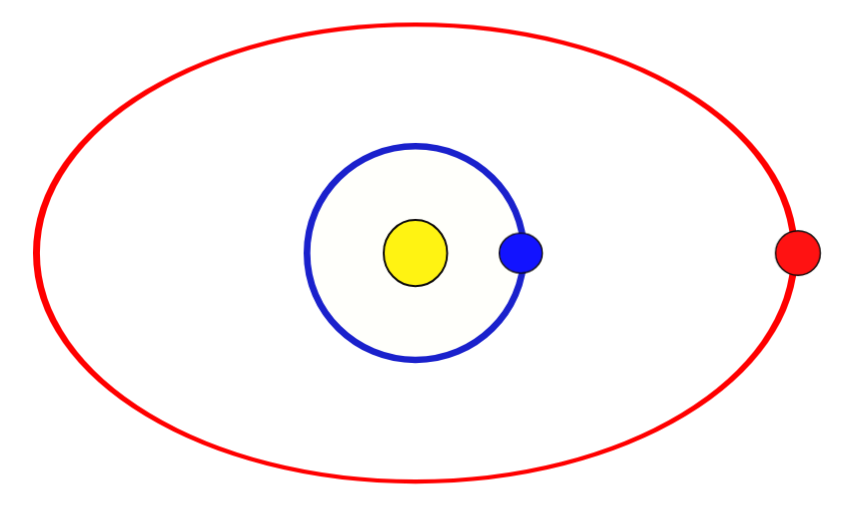
\includegraphics[width=7cm]{Sun_Mars_Orbit} 
    \caption{This is the orbit of Earth and Mars around the Sun.}
    \label{fig:Orbit} 
\end{figure}


\section{Background Researh: }

\subsection{Literature Review: }

\subsection{Symbolic Regression: }

Symbolic regression, is a technique that analyses and searches over the space of traceable mathematical
expressions to find the best fit for a data set. By not requiring prior information about the model,
it is unbiased. There are a plethora of various strategies \cite{lacava2021} that have been implemented in solving for
empirical laws \cite{Schmidt22009}, we will explore some of them below. It is also worth mentioning, that unlike other
well-known techniques for regression, (eg: neural networks), that are essentially black boxes \cite{abroshan2023}, symbolic
regression, aims to extract white-box models and is easy to analyse.\\

\subsubsection{Brute Force: }
Symbolic Regression (SR), is interpretable \cite{Aldeia2022}, unlike Neural Networks (NN), which are often considered more explainable. The difference is interpretability allows us to comprehend how the model works,
like observing how gears move in a glass box, while explainable means you get an overview of why a
certain output was achieved, even without knowing the full nuances of it’s inner workings. This however does not mean there aren't ways to approach this incrementally with neural networks, which allows for interpretability to increase \cite{badiri2020}.\\

There however, are some challenges associated with SR, in comparison to function fitting (NN). SR,
starts with nothing, a blank slate, and it has to learn the entire expression \cite{Cranmer2020}, unlike function fitting
which just tweaks an already existing function. The exponential search space \cite{Worm2014} , causes it to be
extremely computationally expensive to explore all possibilities. This combined with the face that,
most optimisation algorithms expect a smooth search space \cite{Makke2024}, however SR lack’s smooth interpolation, small changes in the potential solutions (expression), ie: $ x3 and x3 + 0.1$ can significantly alter
the the output. Finally, if the nature of the problem is badly posed \cite{Rivero2022}, there might potentially be
multiple solutions to the same data. Imagine trying to find a single polynomial equation with only two
points of data, the need to balance finding accurate expressions with finding the most simplistic and
generalisable fit, is sometimes troublesome.\\

The brute force approach of simply trying all possible combinations of symbolic expressions within some defined space. The model will subsequently increase the complexity over time, and will stop when either the fitting errors lowers below some defined limit or exceeds the upper limit of runtime. While in theory can solve all of our problems, in practise takes longer than the age of our universe to finish. In essence it's like searching for a singular drop in the ocean. Thankfully, there are some ways of pruning the search space, and drastically reducing the time taken to solve for the most accurate expression. \\ 


\subsubsection{Partial Derivatives: }


Partial derivatives, of some function f, with multiple variables such as x and y, is it's dervative with respect to one of those two variables, while the other variables in the function are kept constant. Formally, given a function with two or more variables, $f(x_1, x_2, \ldots, x_n) $, the partial derivative of $f$ with respect to $x_i$, where $x_i$ is some value $x$ in $(x_1, x_2, \ldots, x_i, \ldots, x_n)$, gives the rate of change of $f$ with respect to $x_i$. It is calculated by taking the ith derivative of $f$ with respect to $x_i$, whilst holding the other variables fixed. \cite{Stewart2012} \cite{Smith2012} \\

The partial derivative of a function $f(x,y)$ with respect to $x$ is denoted $\frac{\partial f}{\partial x}$ \cite{Kelly2021} and is defined: \\ 

\begin{center}

  $\frac{\partial f}{\partial x} = \lim_{h \to 0} \left[ \frac{f(x+h, y) - f(x,y)}{h} \right]$
\end{center}


Once you pass in the experimental data, you can pre-process the data, using calculated partial derivatives, for every pair of existing variables. Many physical laws, involve rates of change, and partial
derivatives help us represent them. Furthermore it also guides the search process, as the algorithm can
use the derivative to accurately represent the underlying laws involved. Through comparing how well
the partial derivatives derived through the experimental data compared to the potential expression,
the algorithm can assess the accuracy and feasibility of the expressions involved. This strategy can
even be extended to prune the search space further, this could be achieved through incorporating
knowledge of physics into the constraints for the partial derivatives. These concepts will be illustrated
with an example below.\\

\begin{figure}[h] 
    \centering
    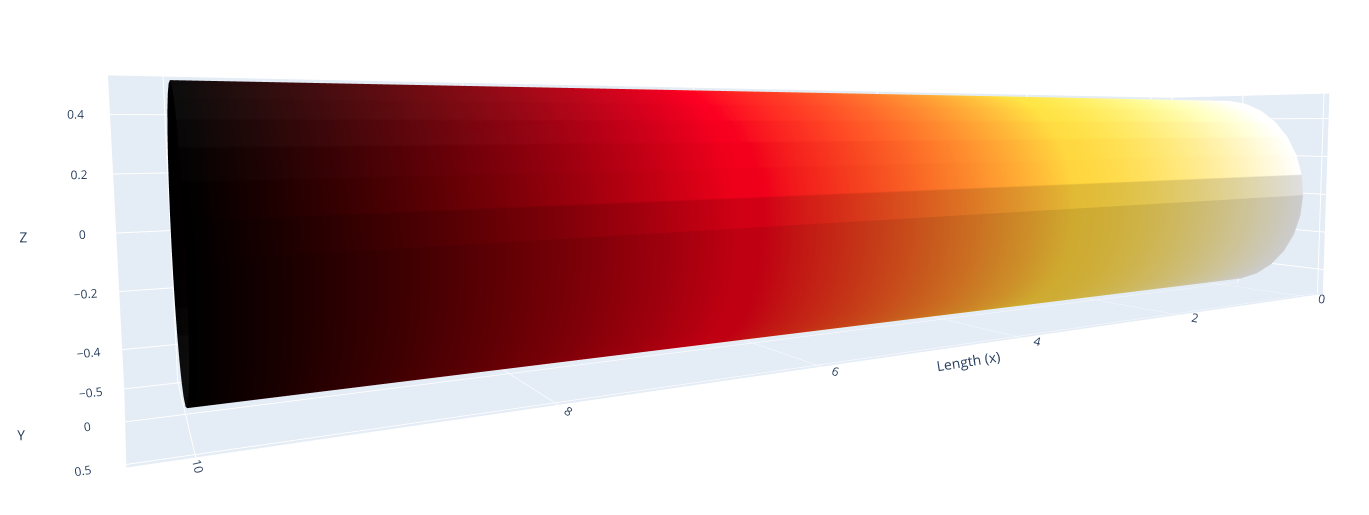
\includegraphics[width=10cm]{heated_rod} 
    \caption{Temperature distribution along a heated rod, illustrating the physical scenario where partial derivatives describe heat flow.}
    \label{fig:Rod} 
\end{figure}





Consider a iron rod, that has been heated up, such that it is hotter on one side than the other. Now it is intuitive to say that closer to the heat source, the temperature will be higher than further along the rod, where it will be colder. We can illustrate this temperature distribution with a function:  \\


\begin{center}
$T(x,y,z)$
\end{center}

where T is the temperature at a point in the rod, and (x,y,z) are the coordinates along the axis in 3 dimensions. This leads to these 3 partial derivatives: \\ 

\begin{center}
 $\frac{\partial T}{\partial x}, \  \frac{\partial T}{\partial y}, \  \frac{\partial T}{\partial z}$
\end{center}

These partial derivatives, gives us information about the direction and magnitude of heat flow at various points on the rod. The algorithm then searches for an equation T(x,y,z), that sufficiently predicts the observed temperature distribution and it's partial derivatives, deriving laws such as the heat transfer equations, or elasticity relationships.\\ 

\begin{center}
$\frac{\partial T}{\partial t} = \alpha \nabla^2 T$
\end{center}



Through using partial derivatives, we have in essence redefined the search criteria for the algorithm, through it's measure of the accuracy in comparison of potential solutions over the invariants represented in the experimental data \cite{Kelly2021} . This also leads to the pleasant finding, that it can additionally capture relationships that represent other identities of the system, beyond invariants and heat transfer equations. \\ 

You can subtly guide the type of laws that such an algorithm finds, by selectively picking the variables to input into the algorithm,. For example providing velocities and force to find laws of motion. \\ 




\subsubsection{Dimensional Analysis: }

Dimensional Analysis is a method of solving problems usually in maths and physics, where we analyse
the relationships between different physical quantities, by comparing their ”units.” It is a powerful
method of reducing the complexity of systems, enabling engineers and scientists to analyse problems
that we can’t even pose, much less solve the equations of \cite{Longo2021}.\\

Using the fact that numerous questions in science can be simplified by requiring the dimensions/units
of the right and left hand side of the expression to be equal, we can transform the question into
a smaller number of variables, which all have no dimension \cite{Blasiak2012}. It has been automated to find the integer powers of expressions and has proven to be useful especially when the power is an irrational number.\\

Here is a general strategy that showcases how dimensional analysis can be used:\\

Let's say we have a variable in an equation that can be broken down into it's fundamental units, such as (second, kilograms, ampere ...) to various powers. We can then take this, and represent each of the units as vectors, such that each of the fundamental units, is assigned a dimension, and it's important to note, this then allows us to represent any physical quantity as a product of these units, so let us construct a vector $v$, with $3$ integers, where each corresponding integer represents the power of each of the fundamental units.\\ 

Given that we want to derive an expression, such as $y = f(x_1, \dots, x_n)$  we can then create some matrix $M$. Each of the columns of the given matrix, is the unit vector $v$ of the corresponding variable $x_i$. We then need to define another vector to represent the units of y, which will be called $z$. If we let the solution be some vector $s$, solving $Ms = z$, this then lets us raise the powers on both sides, to elevate the independent variables, to make this equation dimensionally consistent.\\ 

Taking the null space of the matrix $M$, where $MV = 0$, allows us a basis to create a dimensionless group, allows for a simplification of the problem.\\

This is also more intuitive to understand physical phenomena, the nature of physics comprehension, making this vital in further understanding derived laws, making the process easier to explain and understand \cite{Taber2009}. Therefore, this is a crucial tool, for cultivating a deeper understanding of physics effectively \cite{Tenachi2023}. \\





\subsubsection{Genetic Programming:}



Genetic programming (GP), is a special evolutionary algorithmic technique, where the individuals are seen as programs that evolve, starting for a population, is iteratively "evolved," transforming the populations of individual programs, into other populations. This new generation of programs are created using some genetic operations or survival criteria, \cite{lacava2021}mimicking natural evolutionary condition on earth.\\ 

A very basic overview, shows that genetic programming algorithms, consists of initializing the population \cite{abroshan2023}, then evaluation of the said population through some predefined metrics and functions, followed by selection of the fittest programs based on the score given by the metric, and "genetic operation," such as reproduction, mutation and cross-over. The algorithm then iterates these steps thousands of times, through many generations, and finally terminates once the desired result has been achieved.\\

We can use genetic programming, and tweak the algorithm, and combine it with symbolic regression, to help us derive laws. \\

Consider modelling the various potential formulas as a tree, which is composed of various functions in the nodes. These functions can vary from arithmetic operations  , mathematical functions, or defined unique operators. Then we can program the fitness function \cite{Angeline1994}, and use it to measure how well the given potential expression in the population compares with the given databases, and given the nature of genetic programming, the better performing functions are more likely to be passed down into the next generation. Then after many iterations, we can give the solution with the best performance. \\ 

There are various ways to implement the fitness function, and for example we can use a criteria like this, along with mean squared error \cite{Liddle2009}:\\

\begin{center}
  $V = 2X + N \cdot ln(M/N) $
\end{center}

Here M is the mean squared error, and N is the number of data points, X is the number of parameters used on the genetic programming algorithm. The lower the value of V is, the better the model performs. The performance of this stratergy can then be evaluated with various other metrics, to judge how well the algorithm performs. \\ 





\section{PySR}

This section describes the initial implementation of the symbolic regression models I developed using the PySR library.\\

\subsection{Momentum Laws: }

To generate the dataset, I chose 100 data points, and created two variables mass (M) and acceleration (a), each represented in two dimensions\cite{cranmer2023}. Then the data points were generated using $numpy.random.randn$ function. The force (F), was then calculated to be the produce of these two data sets. Mass and acceleration were concatenated along the same axis using $numpy.concatenate$, resulting in a combined dataset. This is partially because the model used here, $PySRRegressor$ expects a single array as input, and this helps highlight the relationship between these variables to the symbolic regression algorithm.\\ 

Then model performed symbolic regression, configured with 40 iterations along with a customer loss function, taken to be the squred diffrence between the prediction and the target variable. \\ 

\begin{center}
  
  $$
  {\boldsymbol{\mathcal{L}(\hat{x}, x) = (\hat{x} - x)^2}}
$$

\end{center}


The model was trained on this dataset, upon termination, it produced a list of potential candidate formulae, from which I manually identified the correct expression, $F = m \dot a$. \\



\begin{algorithm}[H]
\SetAlgoLined
\KwResult{A symbolic representation approximating \( F = M \cdot A \)}
\textbf{Initialization:} \\
Generate random data for mass (\( M \)) and acceleration (\( A \))\;
Compute target force values: \( F = M \cdot A \)\;
Combine \( M \) and \( A \) into input matrix \( X \)\;

\While{Symbolic regression process}{
  Train the symbolic regression model with the following settings:\;
  \textbf{Binary operators:} Multiplication (\(*\))\;
  \textbf{Unary operators:} None\;
  \textbf{Loss function:} Mean squared error between predictions and targets\;
  \textbf{Iterations:} 40\;

  \eIf{Current symbolic representation improves loss}{
   Update the symbolic model\;
   Save the current best expression\;
   }{
   Continue exploration of new symbolic expressions\;
  }
 }
\caption{Symbolic Regression for \( F = M \cdot A \)}
\end{algorithm}

\\
\\



Similarly, the other laws of momentum, were also dervied using this approach. \\ 



\\

\begin{align} \label{eq:impulse_momentum}
\mathbf{F} \Delta t &= \Delta \mathbf{p} = m(\mathbf{v}_f - \mathbf{v}_i) \\
m_1 \mathbf{v}_{1,i} + m_2 \mathbf{v}_{2,i} &= m_1 \mathbf{v}_{1,f} + m_2 \mathbf{v}_{2,f}
\end{align} 
%\subsection{Optimising the Symbolic Regression Algorithm: }

%\subsection{Neural Networks: }

%\subsection{ White Box models: }

\subsection{Pendulum Laws:}

The data is generated using numpy. The simulation involves, Euler's method to solve the pendulum's equation of motion. Through taking small and discrete steps, the method approximates the solution. The equation for a simple pendulum is given by: \\



\begin{center}
\begin{equation}
\alpha = -\frac{g}{L} \sin(\theta)
\end{equation}
\end{center}

\begin{description}
    \item[\(\alpha\)] angular acceleration (\(\text{rad/s}^2\))
    \item[\(g\)] acceleration due to gravity (\(\text{m/s}^2\))
    \item[\(L\)] length of the pendulum (\(\text{m}\))
    \item[\(\theta\)] angular displacement (\(\text{rad}\))
\end{description}

The Euler technique approximates the changes in angular velocity and displacement over some small step in time, as follows:\\

\begin{center}
\begin{align} 
\omega_{i+1} &= \omega_i + \alpha_i \Delta t \\
\theta_{i+1} &= \theta_i + \omega_{i+1} \Delta t 
\end{align}
\end{center}


The function iterates through a few hundred time steps, updating the angular velocity and displacement at each time step. To prevent errors accumulating due to numerical drift, which are small errors that accumulate and become significant due to the inherent nature of approximation methods like Eulers. To keep the values coherent, a wrap around operation is used to ensure the angular displacement is within the range of [\pi, -\pi] radians.\\ 

\begin{figure}[H]
    \centering
    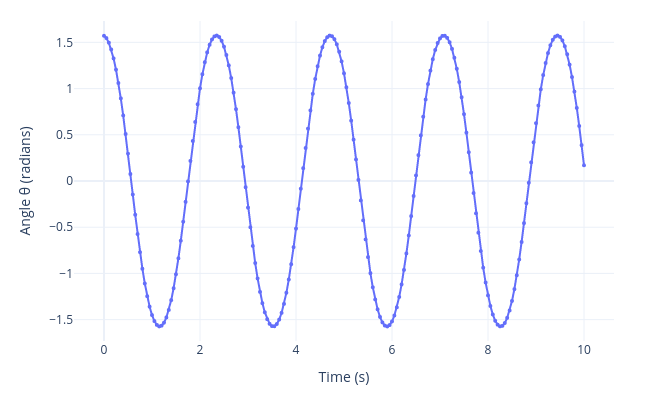
\includegraphics[width=8cm]{pendulum_simulation}
    \caption{The motion of a simple pendulum using the Euler method.} % Optional
    \label{fig:sr_flow}
\end{figure}



\subsection{Noise: }


This section investigates the model's robustness to noise. To simulate varying levels of interference, artificial noise was systematically introduced during the data generation phase, building upon the previously established model framework. Noise was modeled by generating random numbers within a range of progressively increasing magnitude, utilizing Python's random library. The objective was to observe and quantify the degradation in model accuracy as a function of increasing noise levels, as well as to explore methods for mitigating its impact.\\



\subsubsection{How noise affects the model: }

To introduce noise into the generated dataset, Python’s \texttt{random} library was used in conjunction with the \texttt{randint} function. An auxiliary function was implemented to systematically increase the parameters passed to \texttt{randint}, resulting in each successive dataset exhibiting progressively higher levels of noise.\\

Following the generation of these noisy datasets, the symbolic regression model was applied to each, and the resulting equations were analyzed. The relationship between noise level and model performance was visualized through a graph. Furthermore, the \texttt{time} library was utilized to measure the execution duration of each model run.\\






\begin{figure}[H]
    \centering
    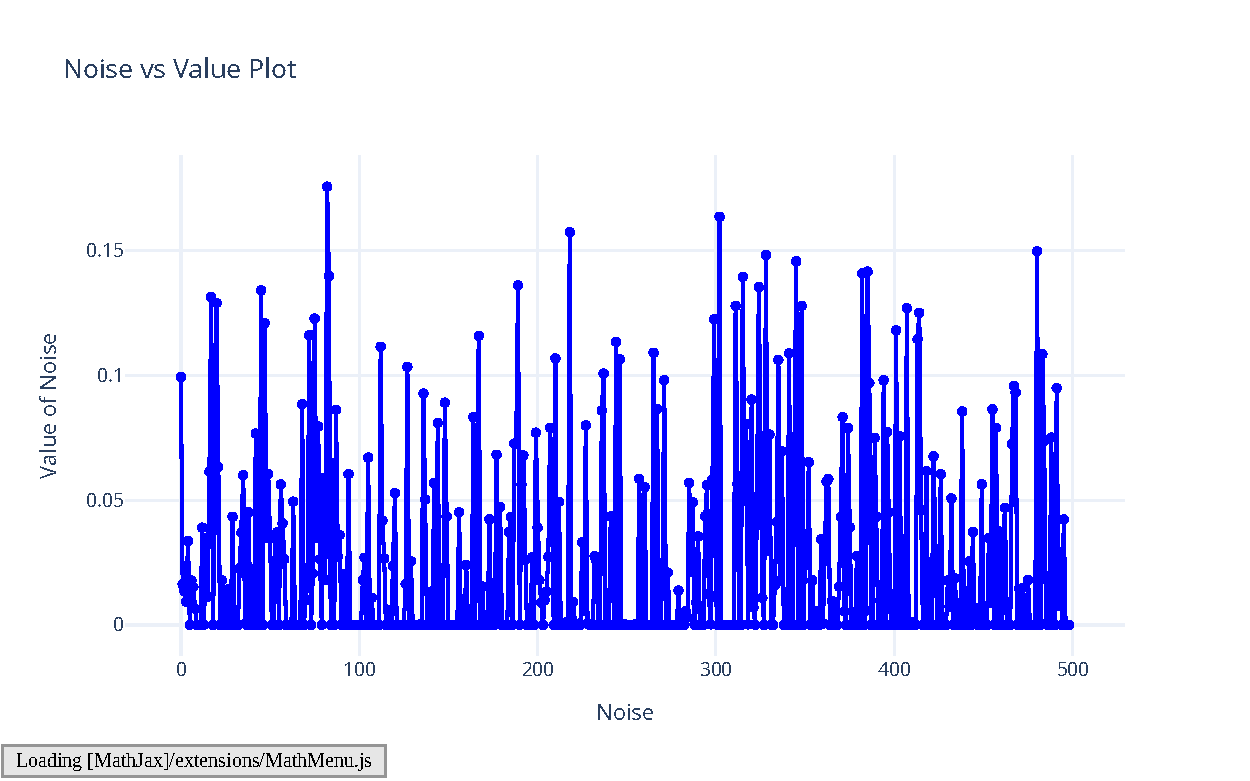
\includegraphics[width=7cm]{noise_conservation_random}
    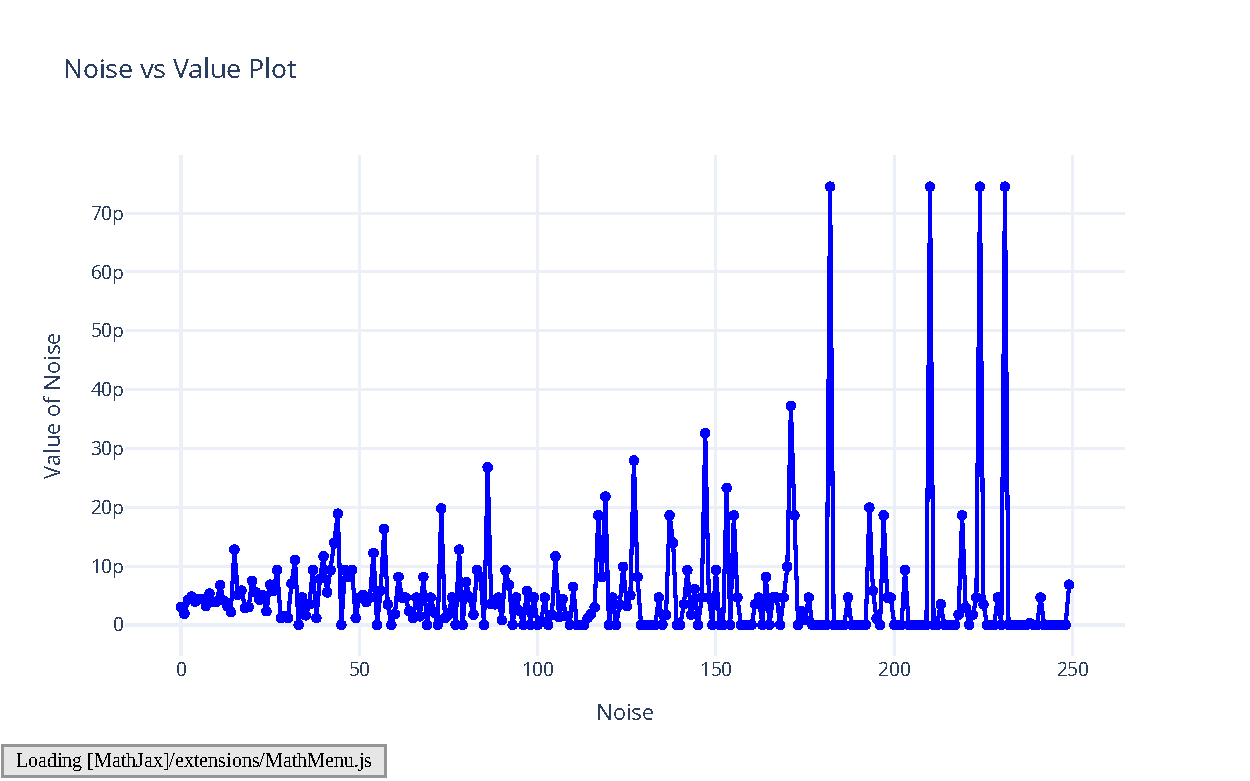
\includegraphics[width=7cm]{noise_Newtons_First_Law_random}
    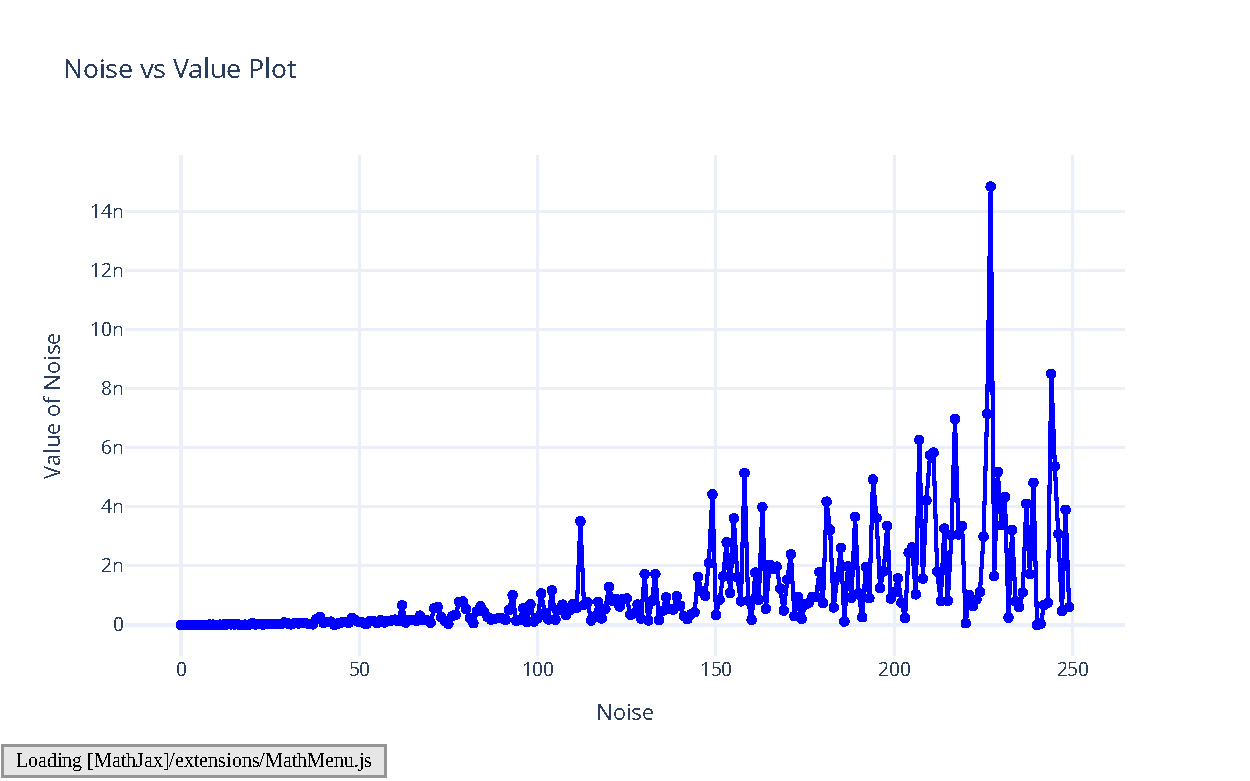
\includegraphics[width=7cm]{noise_Newtons_Third_Law_random}
    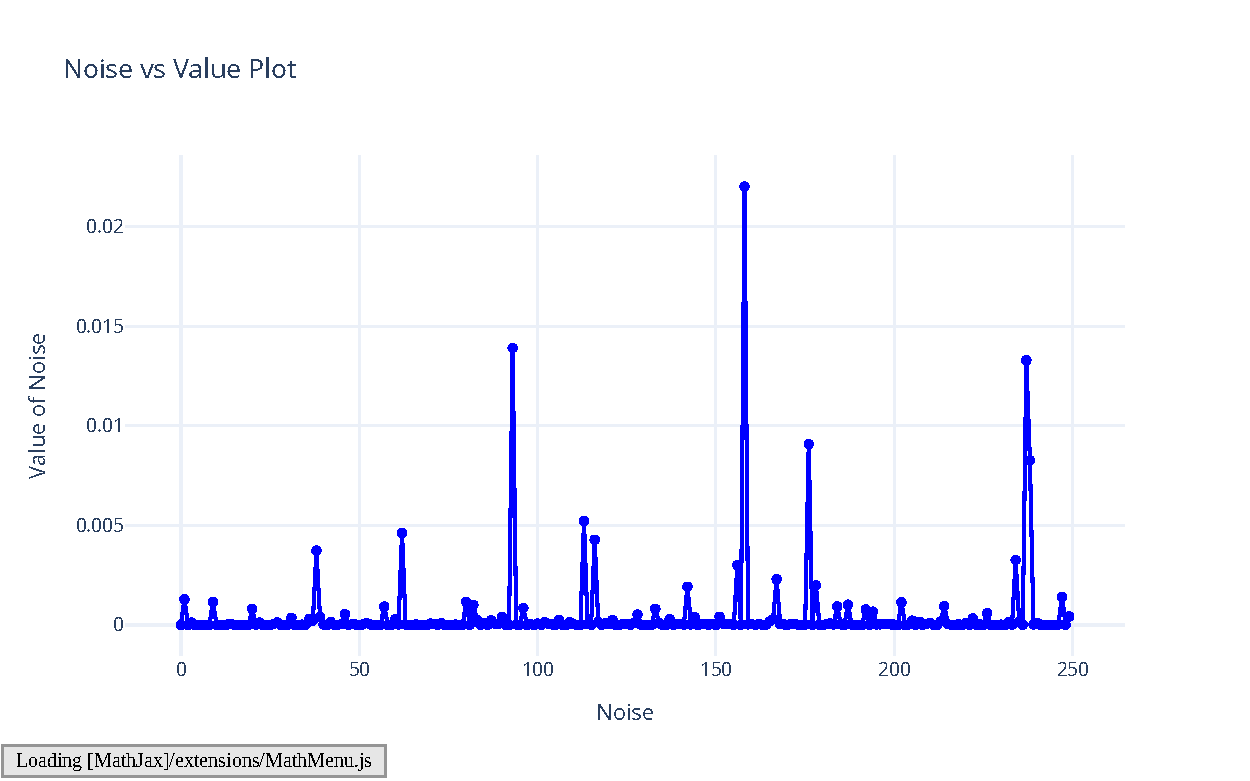
\includegraphics[width=7cm]{noise_Simple_Harmonic_Motion}
    \caption{Plots showing how loss behaves as noise is increased randomly.}
    \label{fig:noise_plots}
\end{figure}

Displays, from top left to bottom right, the principles of Conservation, Newton's First Law, Newton's Third Law, and Simple Harmonic Motion.\\

This is the iterative model, where noise is increased iteratively (not random).\\ 

\begin{figure}[H]
    \centering
    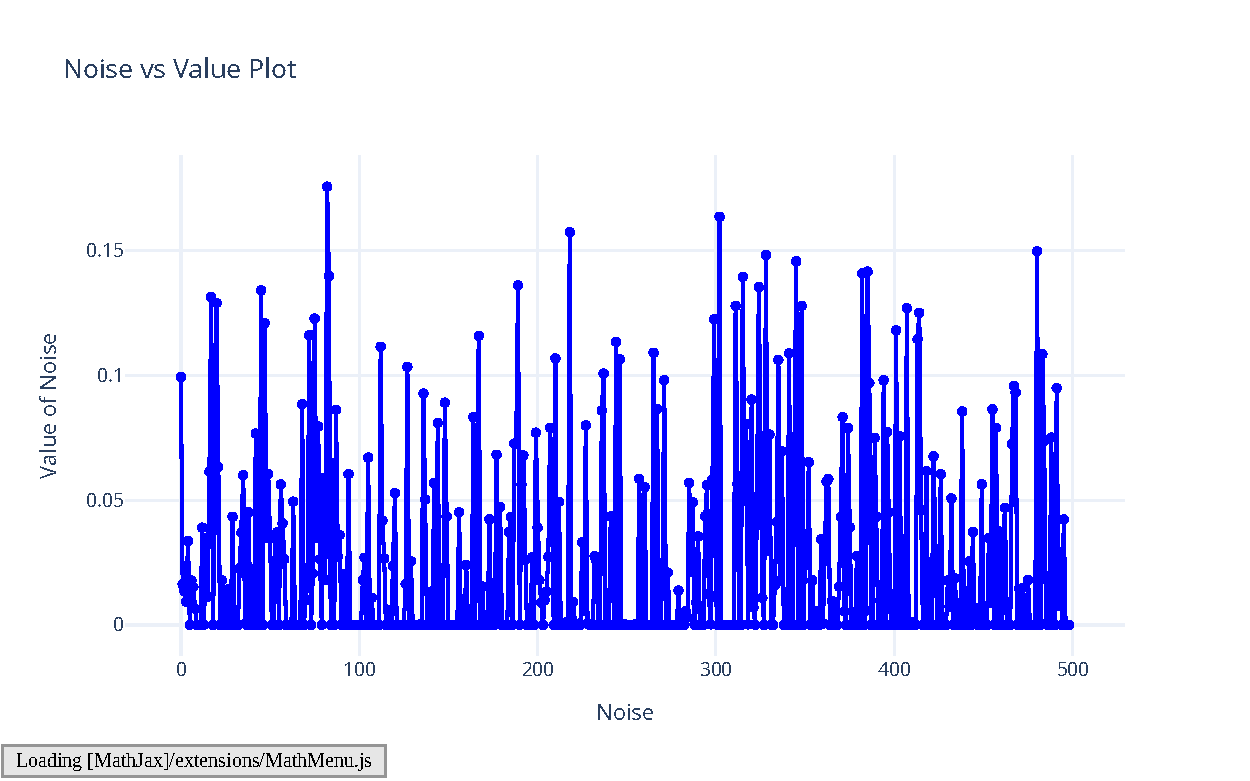
\includegraphics[width=7cm]{noise_conservation_random_i}
    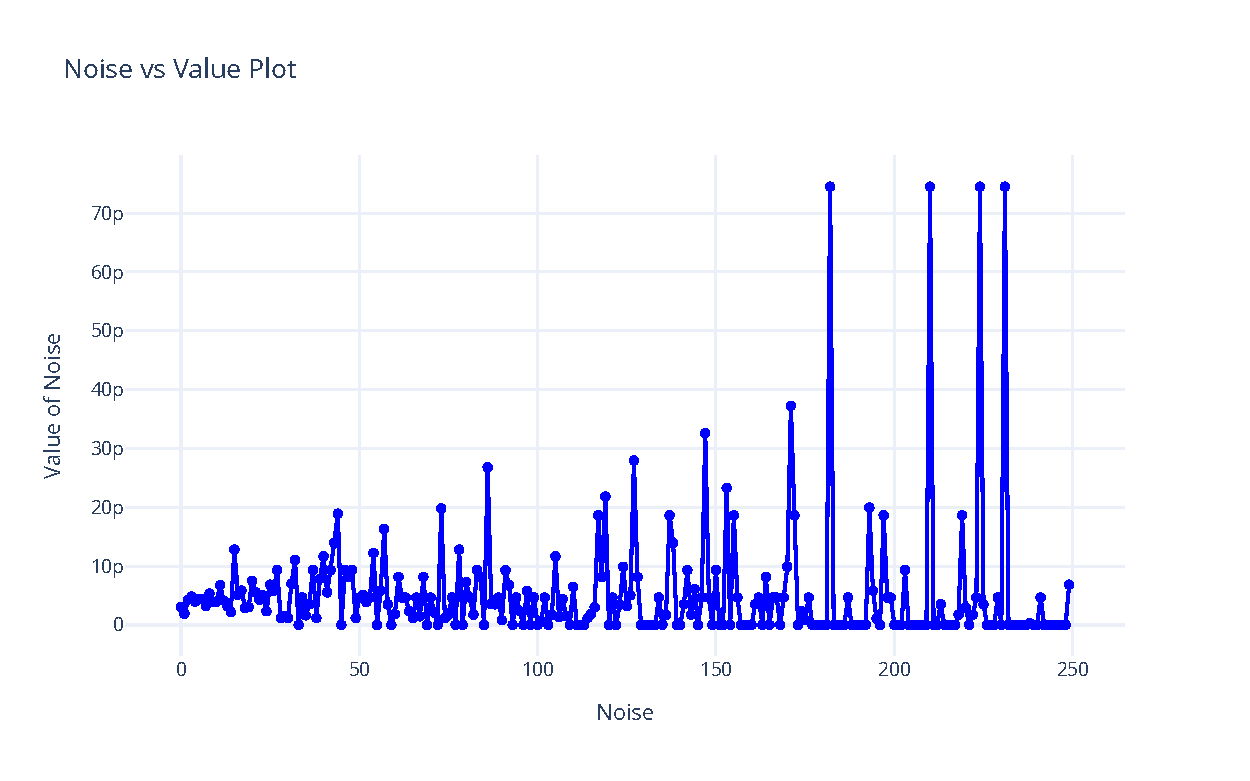
\includegraphics[width=7cm]{noise_Newtons_First_Law_random_i}
    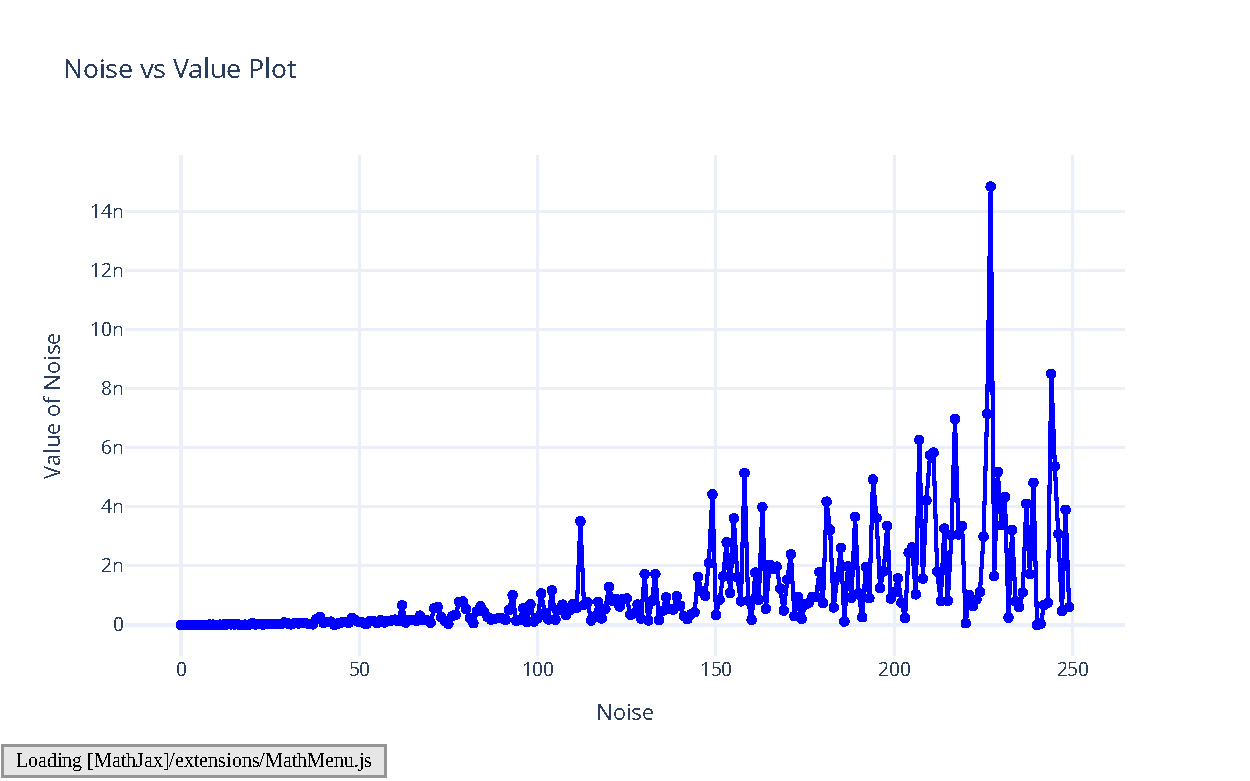
\includegraphics[width=7cm]{noise_Newtons_Third_Law_random_i}
    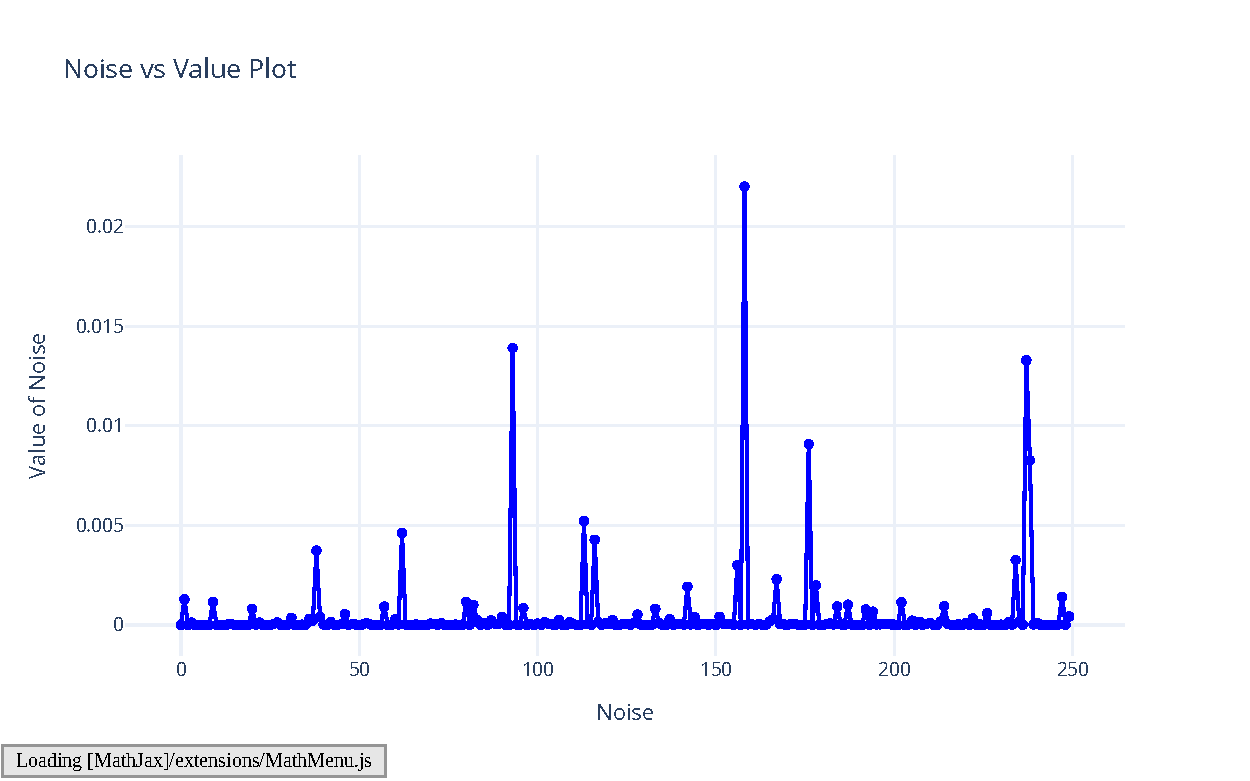
\includegraphics[width=7cm]{noise_Simple_Harmonic_Motion_random_i}
    \caption{Plots showing how loss behaves as noise is increased iteratively.}
    \label{fig:noise_iterative_plots}
\end{figure}


\subsubsection{Denoise function: }

Following the initial noise analysis, a subsequent experiment introduced a denoising method—implemented using a Python library—applied to the data prior to processing by the PySR model. The results, as shown in the accompanying plot, demonstrate that this denoising approach enhanced model performance up to a specific noise threshold. However, beyond this critical level, performance deteriorated similarly for both the denoised and non-denoised datasets, indicating that the effectiveness of the denoising function diminished at higher noise intensities.\cite{Wood2022} \\



\begin{figure}[H]
    \centering
    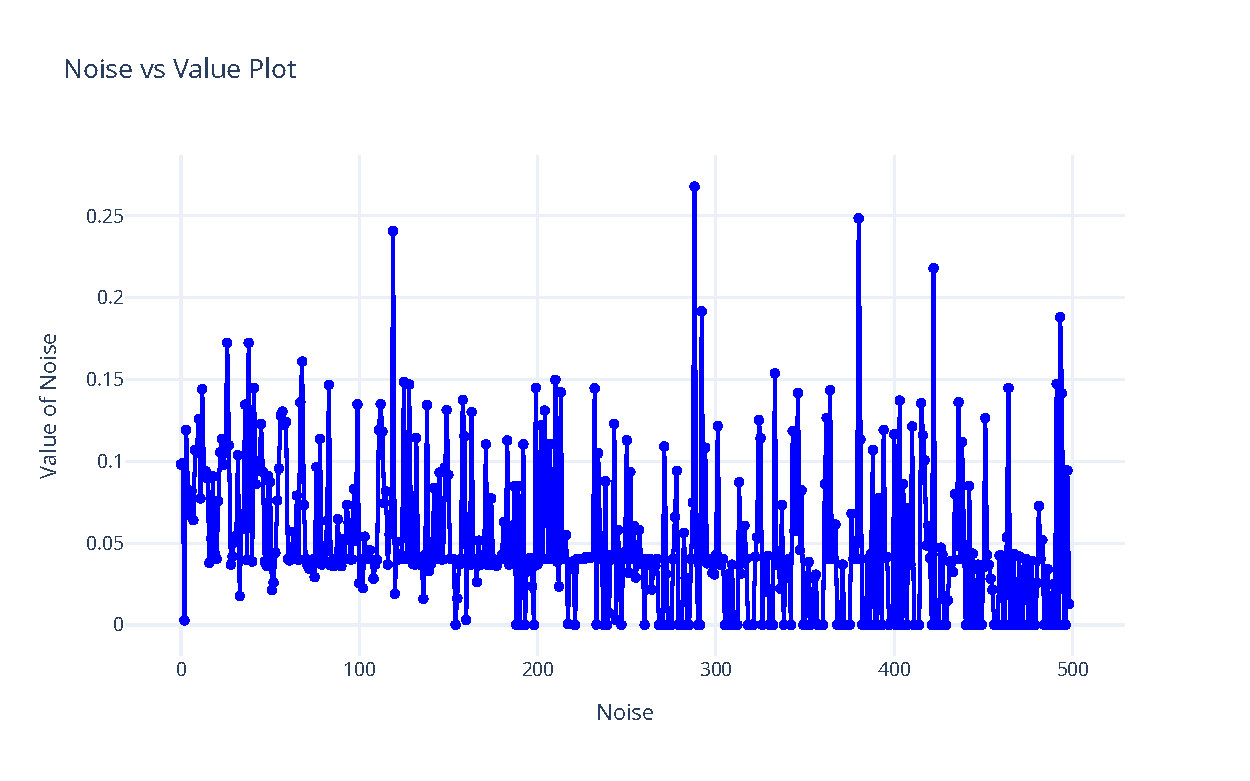
\includegraphics[width=7cm]{noise_conservation_d_r}
    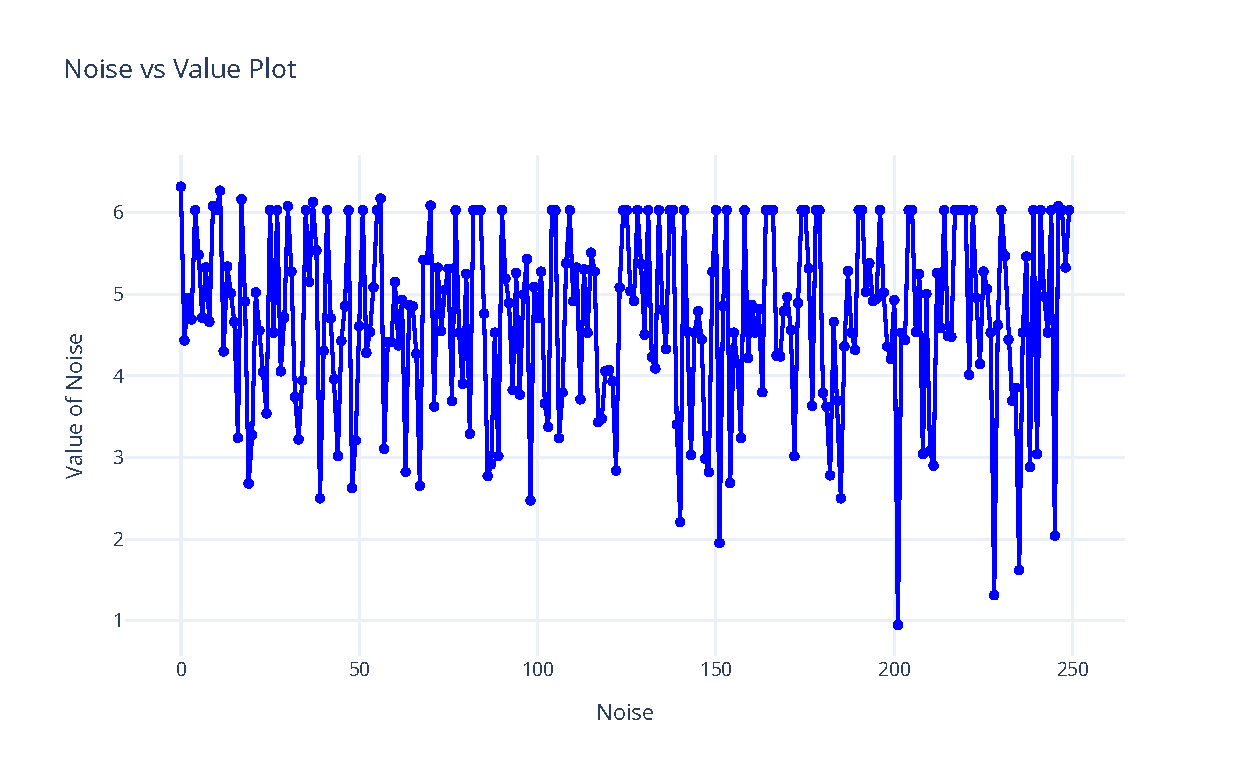
\includegraphics[width=7cm]{noise_Newtons_First_Law_d_r}
    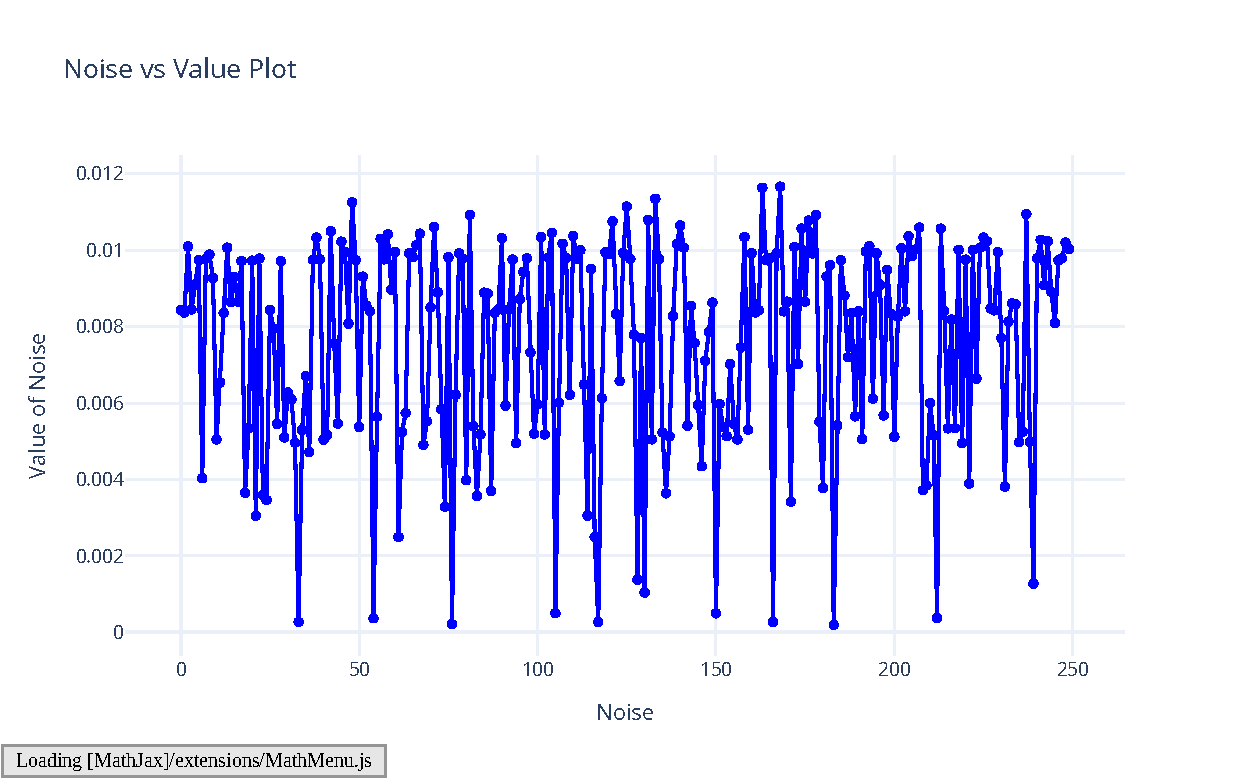
\includegraphics[width=7cm]{noise_Newtons_Second_Law_d_r}
    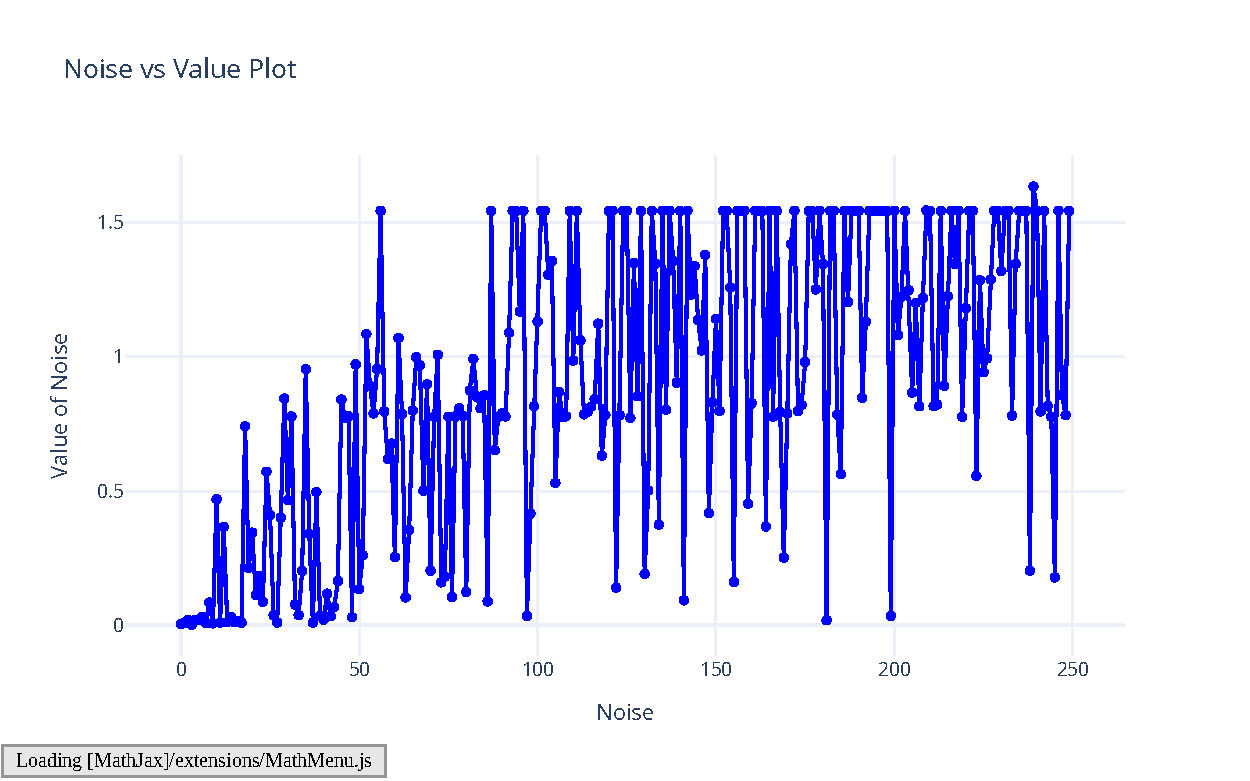
\includegraphics[width=7cm]{noise_Newtons_Third_Law_d_r}
    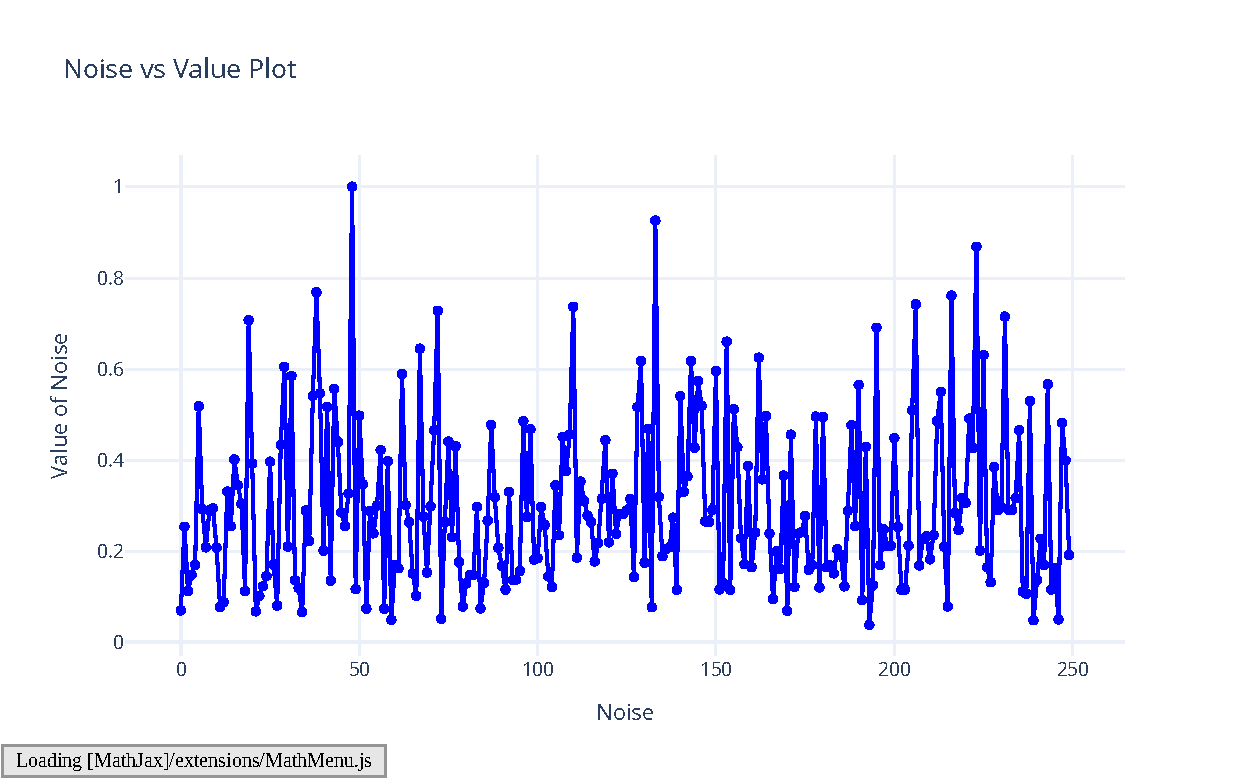
\includegraphics[width=7cm]{noise_Rutherford_d_r}
    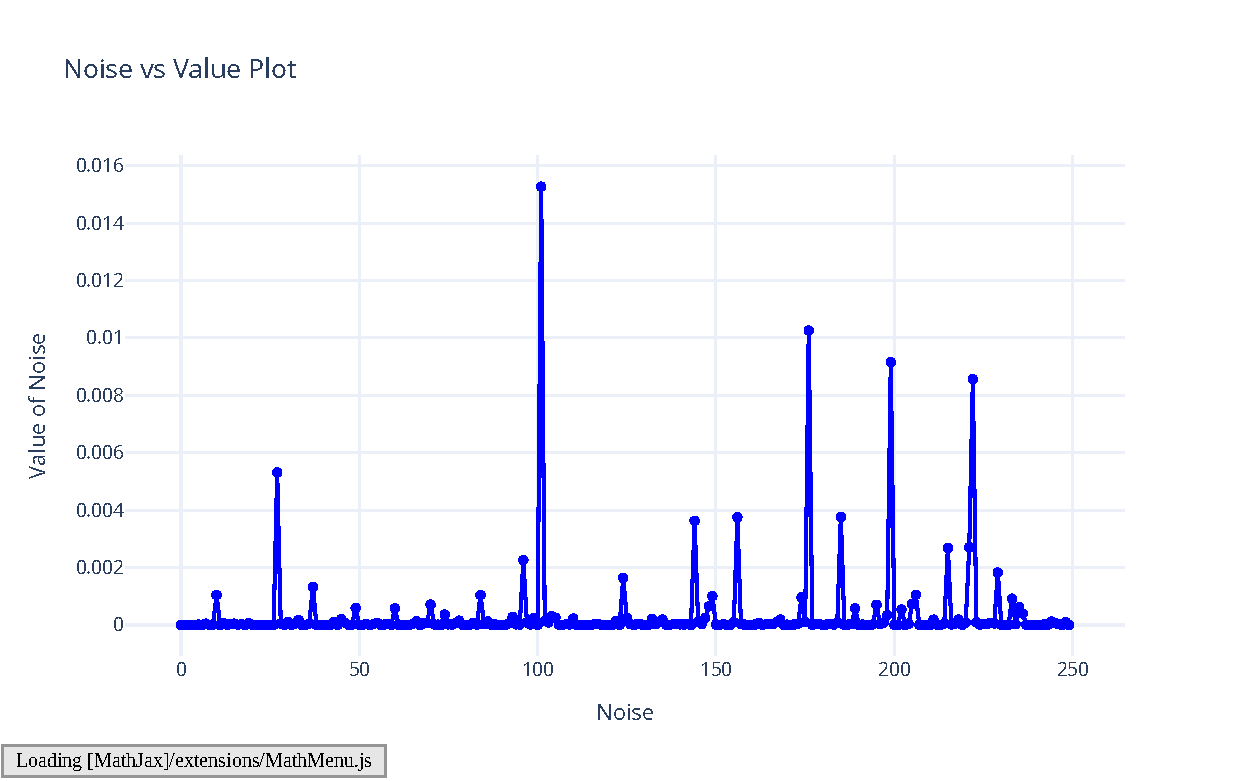
\includegraphics[width=7cm]{noise_Simple_Harmonic_Motion_d_r}
    \caption{Noise plots with dimensionless reduction for various physical systems.}
    \label{fig:noise_dimless_plots}
\end{figure}

From top left to bottom right, the diagram illustrates the laws of Conservation, Newton's First Law, Newton's Second Law, Newton's Third Law, Rutherford's Model, and Simple Harmonic Motion.\\
This is the iterative model, where noise is increased iteratively (not random).\\ 


\begin{figure}[H]
    \centering
    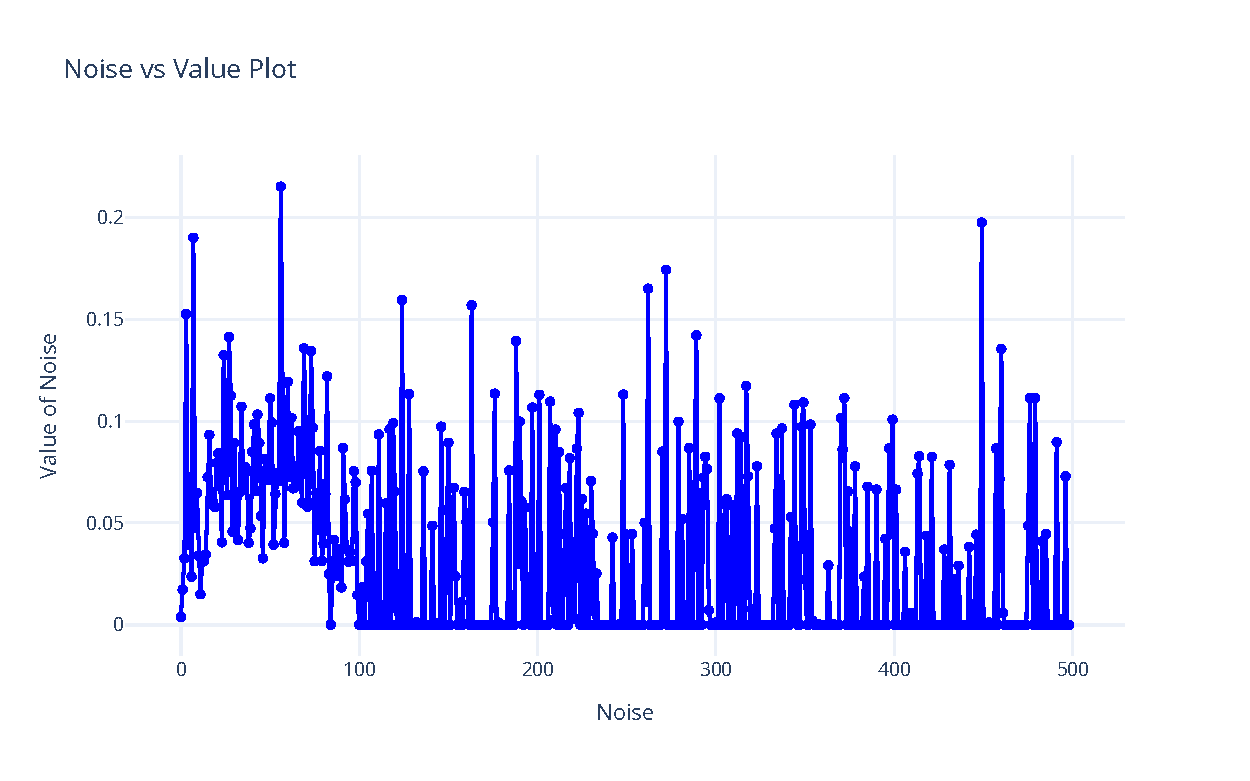
\includegraphics[width=7cm]{noise_conservation_d_i}
    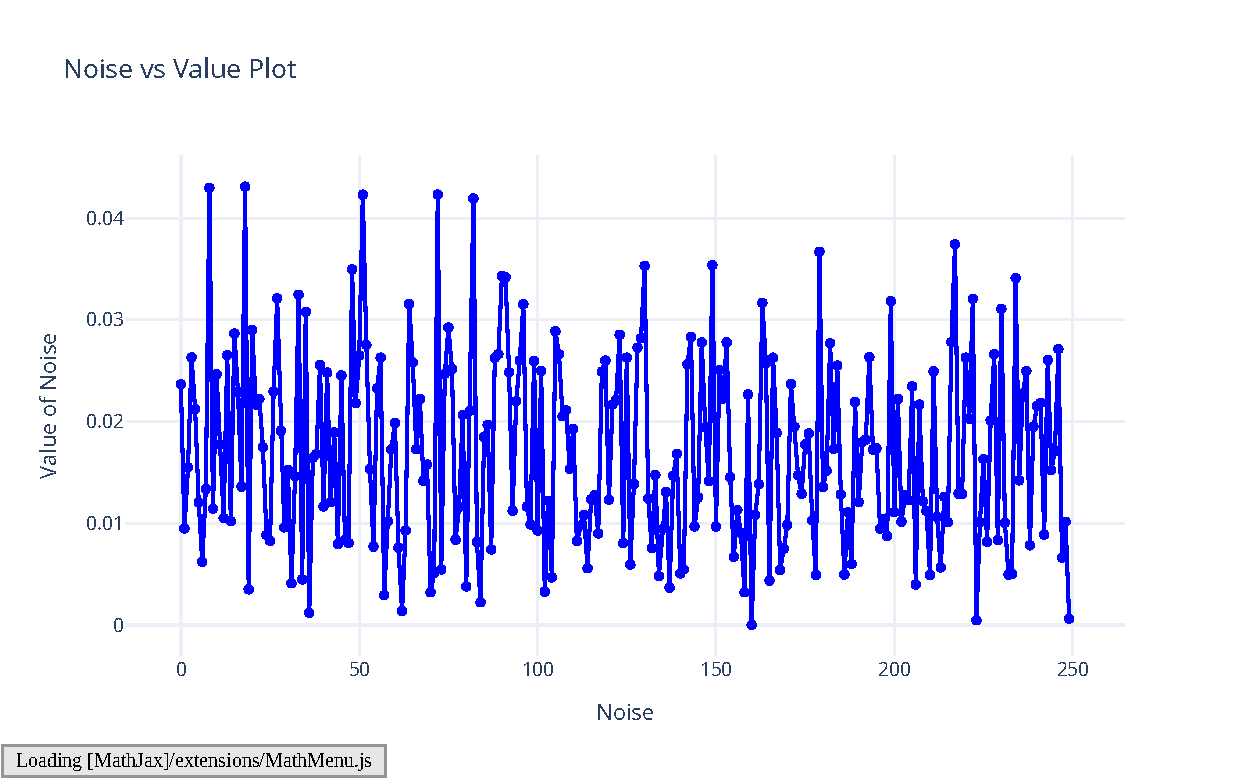
\includegraphics[width=7cm]{noise_Newtons_First_Law_d_i}
    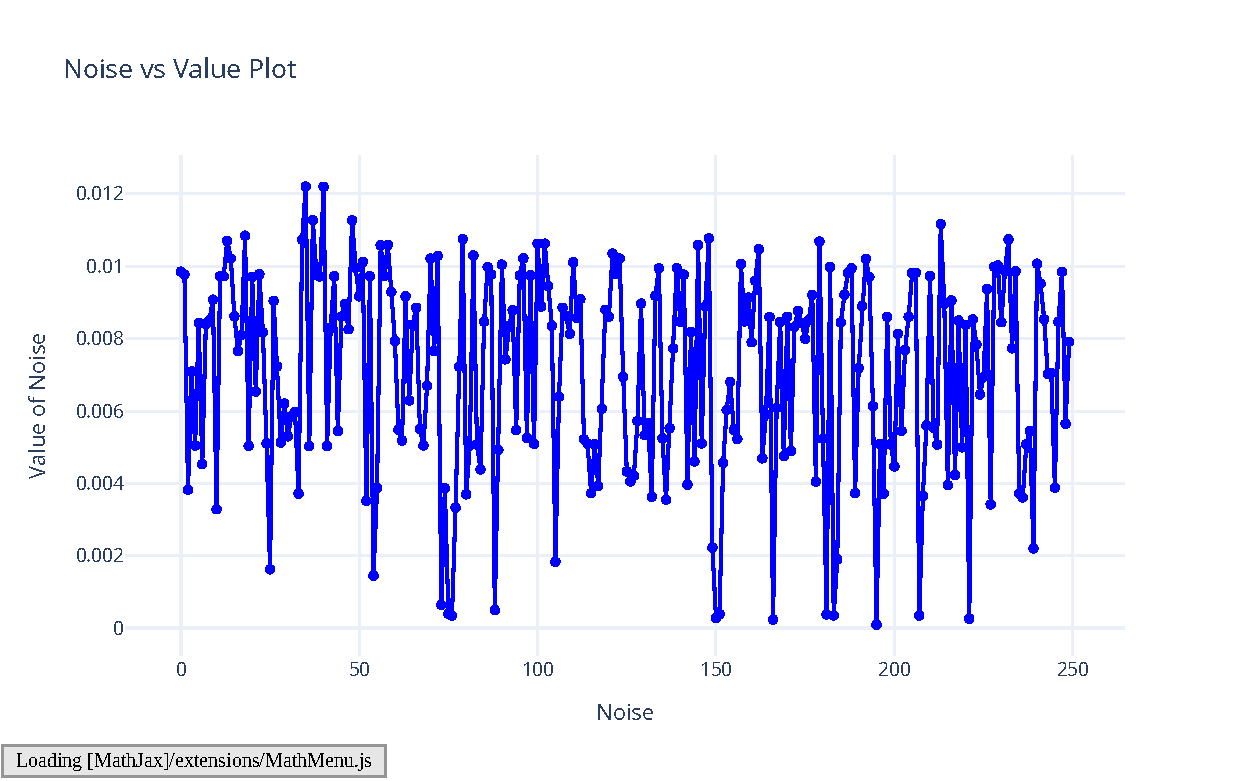
\includegraphics[width=7cm]{noise_Newtons_Second_Law_d_i}
    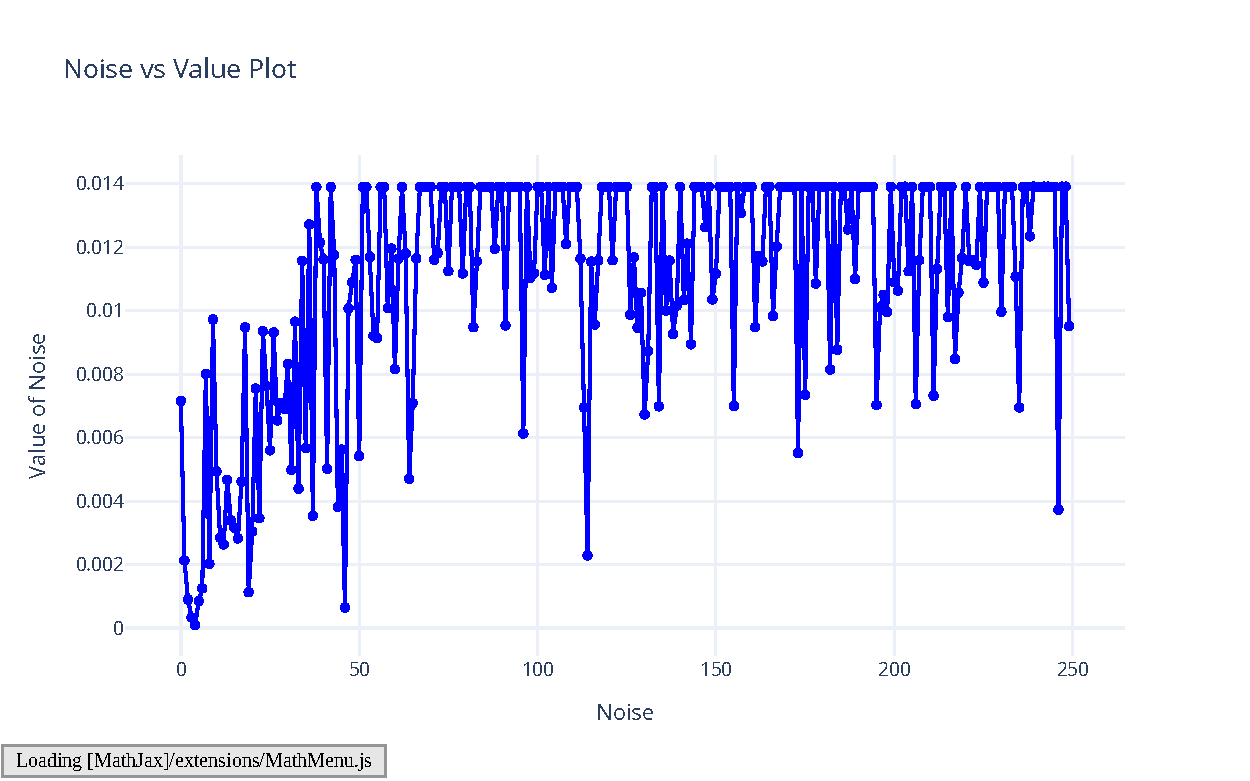
\includegraphics[width=7cm]{noise_Newtons_Third_Law_d_i}
    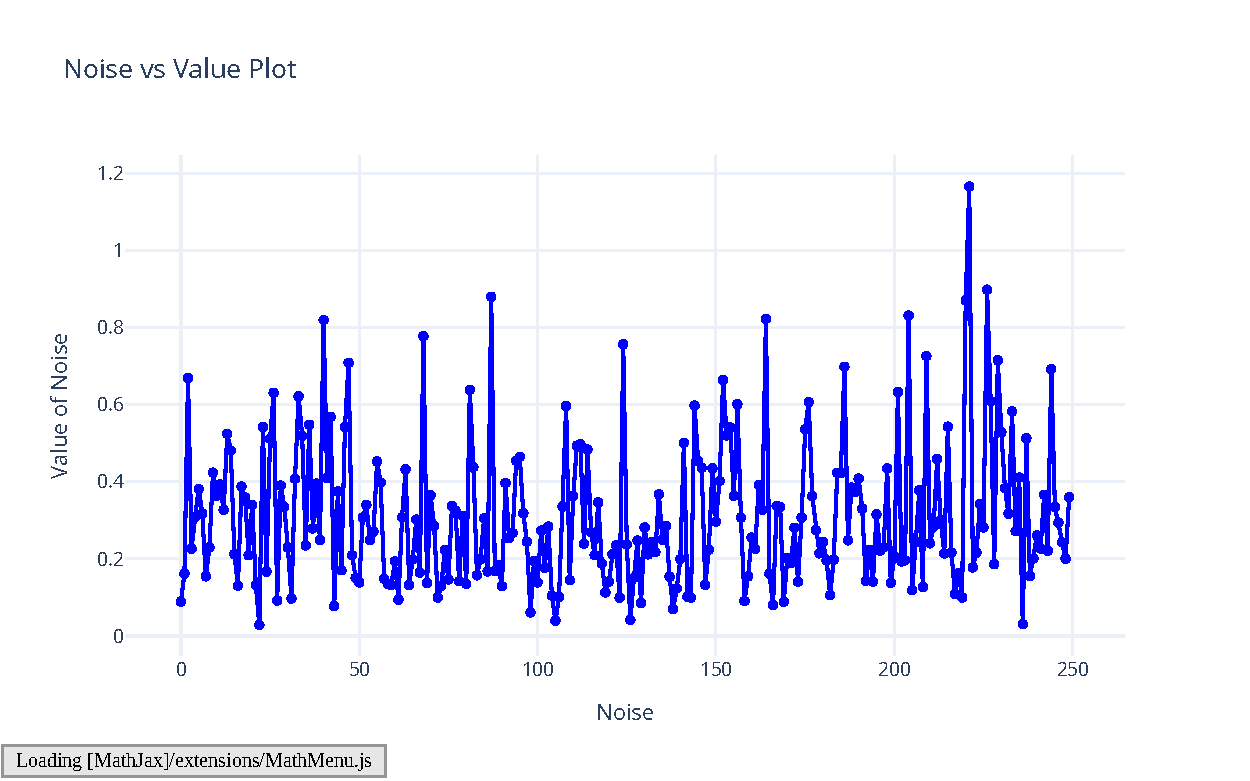
\includegraphics[width=7cm]{noise_Rutherford_d_i}
    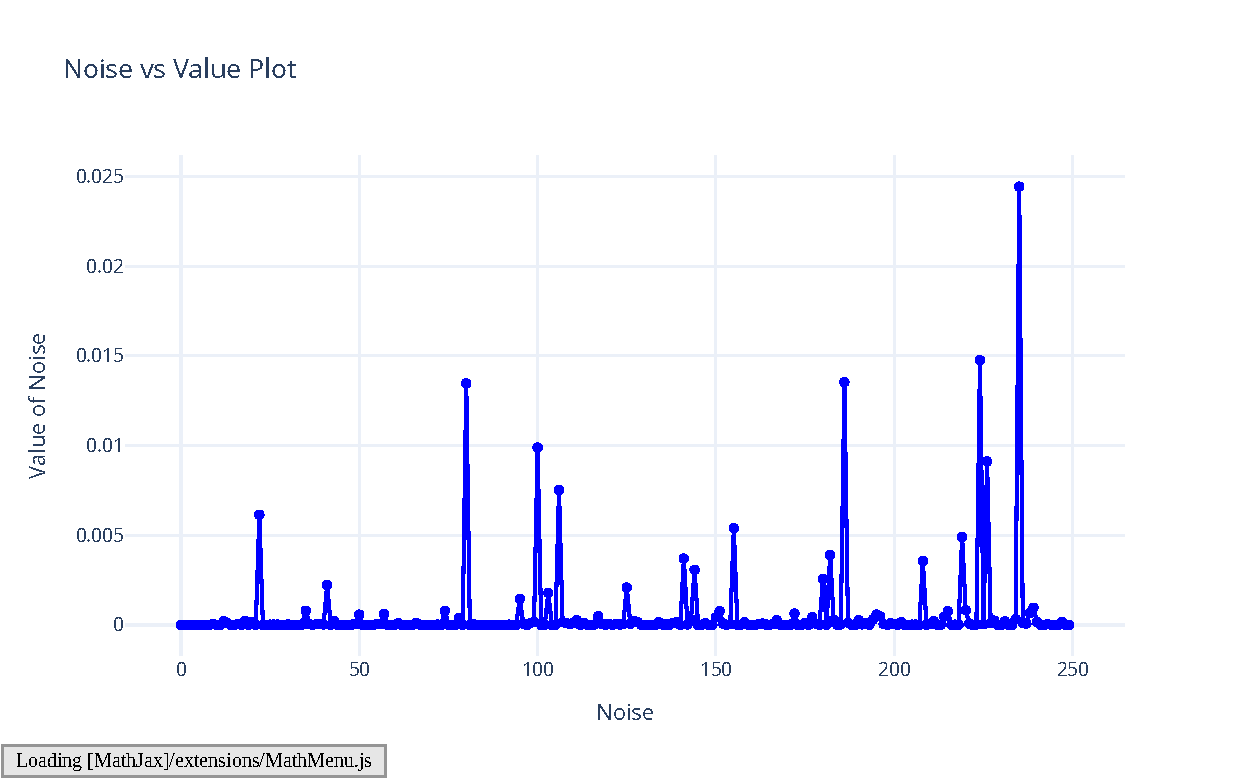
\includegraphics[width=7cm]{noise_Simple_Harmonic_Motion_d_i}
    \caption{Noise plots with dimensionless reduction and iterative improvement for various physical systems.}
    \label{fig:noise_dimless_iterative_plots}
\end{figure}





\section{Symbolic Regression from First Principles: }


\subsection{A Brute-Force Approach: }

The core and essential component of any symbolic regression model lies in its ability to generate and traverse the search space of potential equations and expressions that best fit the given data. To streamline this process and validate the functionality of expression generation, simple two-variable equations were initially implemented, with specified operations used within each equation. This approach was first limited to basic operations, with future extensions planned to incorporate constants and additional complexities.\\



\begin{algorithm}[H]
\SetAlgoLined
\KwData{List of variable names, list of constants, list of operators}
\KwResult{List of generated symbolic expressions}

\textbf{Initialization:}\;
Create pool of symbolic variables and constants from inputs\;
Initialize empty list for expressions\;

\For{each pair (a, b) from the pool (considering permutations)}{
  \For{each operator op from the list of operators}{
    Form expression \( a \text{ op } b \)\;
    \If{resulting expression is valid}{
      Add expression to the list of expressions\;
    }
  }
}

Return list of expressions\;

\caption{Generate Initial Symbolic Expressions}
\label{alg:generate_expressions} % You can use this label to reference the algorithm
\end{algorithm}\\


Subsequently, this approach was refined by designing a recursive method for generating expressions, enabling the creation of more robust and diverse equations from the available variables. This process is dynamic and adaptable to a wide range of input configurations.\\




\begin{algorithm}[H]
\SetAlgoLined
\KwData{List of operators, list of variable names, maximum depth}
\KwResult{List of symbolic expressions generated at the maximum depth}

\textbf{Initialization:}\;
Create list `Expressions[0]` containing symbolic variables from input\;

\For{depth \(d\) from 1 to maximum depth}{
  Create empty list `Expressions[d]`\;
  \For{each expression \(a\) in `Expressions[d-1]`}{
    \For{each expression \(b\) in `Expressions[d-1]`}{
      \For{each operator \(op\) in list of operators}{
        Attempt to form new expression \( a \text{ op } b \)\;
        \If{resulting expression is valid}{
          Add new expression to `Expressions[d]`\;
        }
      }
    }
  }
}

Return `Expressions[maximum depth]`\;

\caption{Recursive Generation of Symbolic Expressions}
\label{alg:recursive_expressions} % Add a label for referencing
\end{algorithm}\\


\subsubsection{ Exploiting Physical Properties: }


The next step involves truncating the generated expressions to prune the search tree as efficiently as possible. An effective method for achieving this is by leveraging the symmetrical properties of physical equations and recognizing their mathematical equivalence. This includes removing redundant or duplicate expressions that do not contribute new information.\\

The following approach was used to implement this:\\



\subsubsection{Dealing with constants:}

Another approach used to further prune the set of generated expressions involved filtering out any expressions that did not contain all the specified variables. This step optimizes the process by reducing the number of irrelevant expressions, ultimately conserving computation time during the evaluation phase.\\



\subsubsection{Dealing with powers:}

To incorporate powers into the expressions, the power operation was integrated directly into the generated equations. This approach not only enables the creation of more complex models but also facilitates the pruning of the search tree by preventing the generation of redundant expressions that already include powers.\\




\begin{algorithm}[H]
\SetAlgoLined
\KwData{List of initial expressions, list of powers, maximum depth}
\KwResult{List of unique symbolic expressions generated by applying powers}

\textbf{Initialization:}\;
Create set `ResultExpressions` and add all initial expressions to it\;

\For{depth \(d\) from 1 to maximum depth}{
  Create empty set `NewExpressionsThisDepth`\;
  \For{each expression \(e\) in `ResultExpressions` (from previous depths)}{
    \For{each power \(p\) in list of powers}{
      Attempt to calculate \( powered\_e = e^{p} \)\;
      \If{resulting expression is valid}{
        Add \( powered\_e \) to `NewExpressionsThisDepth`\;
      }
    }
  }
  Add all expressions from `NewExpressionsThisDepth` to `ResultExpressions`\;
}


\caption{Apply Powers Recursively to Expressions}
\label{alg:apply_powers} % Add a label for referencing
\end{algorithm}\\




A filtering mechanism was implemented based on whether the expression included a power operation. This further reduces the size of the search tree by removing unnecessary branches. Although a more robust model could derive the power operation from scratch, this approach was chosen to optimize computation time and maintain flexibility.\\

\begin{algorithm}[H]
\SetAlgoLined
\KwData{List of expressions, list of target powers}
\KwResult{List of expressions containing a sub-expression with a target power}

\textbf{Initialization:}\;
Create empty list `FilteredExpressions`\;

\For{each expression \(e\) in input expressions}{
  Set `found_target_power` to false\;
  Traverse the symbolic tree of \(e\) (e.g., preorder)\;
  \For{each sub-expression \(s\) during traversal}{
    \If{\(s\) is a power AND exponent of \(s\) is in target powers}{
      Set `found_target_power` to true\;
      Break traversal for \(e\)\; % Stop searching this expression
    }
  }
  \If{`found_target_power` is true}{
    Add \(e\) to `FilteredExpressions`\;
  }
}

Return `FilteredExpressions`\;

\caption{Filter Expressions by Presence of Target Powers}
\label{alg:filter_powers} % Add a label for referencing
\end{algorithm}



\subsubsection{Chaining powers and constants:}

The following step involved chaining together powers and constants, applying both to the generated expressions. While the existing design already supports chaining, it was crucial to properly filter the results to ensure the search tree remained as compact as possible.\\

Although constants can be filtered using the existing method, the power operations are embedded within the constants, which caused the previous power filter to no longer function as expected. As a result, the filtering process was redesigned to operate recursively, allowing it to handle both powers and constants effectively.\\

Nevertheless, this approach occasionally produces expressions that contain chained constants, such as sin(sin()). To enhance the model further, an additional filter was introduced to eliminate expressions with multiple instances of the same constant chained together.\\


\subsubsection{Loading data:}


The next step was to implement an efficient method for loading the generated data. Since rapid testing was a priority at this stage, dummy data values were initially created. To optimize performance, the data was stored as a NumPy array, offering significant speed advantages over text files. This choice was driven by several factors, including the in-memory storage of NumPy arrays, the efficiency of the underlying binary data format, and the use of C in NumPy, which enables the vectorization of operations.\\





\begin{algorithm}[H]
\SetAlgoLined
\KwData{Input matrix \(X\), target vector \(Y\), list of variable names}
\KwResult{Input matrix \(X\), target vector \(Y\), list of symbolic variables}

\textbf{Check Input Validity:}\;
\If{number of columns in \(X\) \(\neq\) number of variable names}{
  Indicate error or stop execution\;
}

\textbf{Process Variables:}\;
Create list of symbolic variables from the list of variable names\;

Return \(X\), \(Y\), and the list of symbolic variables\;

\caption{Load and Validate Data}
\label{alg:load_data} % Add a label for referencing
\end{algorithm}\\



As demonstrated, a check is performed to ensure that the number of variables provided matches the shape of the array X, where X represents the input data and y represents the target data, i.e., the final result. For instance, X contains the mass and acceleration values, while y contains the corresponding force values f, calculated using the equation f=ma. This check serves as a basic validation to confirm that the number of columns in the input data aligns correctly with the variables provided.\\


\subsubsection{How to mitigate noise in data: }

Ways to mitigate noise and its effects on the model were explored. Functions such as "denoise" in the symbolic regression library provided some improvements. However, beyond a certain point, these methods did not appear to offer significant assistance.\\

Additionally, a custom denoising algorithm was developed, implementing several different techniques to assess their impact. The first approach involved using a simple moving average to reduce noise in the dataset.\\

The moving average method is both simple and fast, effectively smoothing data by averaging neighboring values. However, it has limitations: while it works well for reducing noise, it blurs sharp transitions and is highly sensitive to extreme outliers. These outliers can pull the average significantly, thereby distorting the signal and impacting the overall accuracy of the model.\\


\subsubsection{Evaluating expressions:}

The generated expressions are evaluated by assigning the input variables to the corresponding columns of the data in increasing order. These values are then substituted into the expressions, and the model performs the calculations, producing an array of outputs for each expression. This process involves evaluating every pruned expression and returning a NumPy array of results based on the input data.\\




\begin{algorithm}[H]
\SetAlgoLined
\KwData{Symbolic expression, list of variable names, input data matrix \(X\)}
\KwResult{Numerical evaluation of the expression for each data point in \(X\), or NaN if evaluation fails}

\textbf{Initialization:}\;
Create list of symbolic variables from the list of variable names\;

\textbf{Convert to Numerical Function:}\;
Convert the symbolic expression into a numerical function, mapping symbolic variables to input columns of \(X\)\;

\textbf{Evaluate:}\;
Prepare input data from columns of \(X\) to match function arguments\;
\Try{
  Evaluate the numerical function using the prepared input data\;
  Return the resulting array of values\;
}
\Catch{Evaluation fails (e.g., division by zero)}{
  Return an array of Not-a-Number (NaN) values with the same size as the number of data points\;
}

\caption{Evaluate Symbolic Expression Numerically}
\label{alg:evaluate_expression} % Add a label for referencing
\end{algorithm}\\



Following the approach outlined in the paper \cite{Liddle2009}, a medium error description length loss function was utilized, implemented as described. The error is calculated using the squared difference to ensure all errors are positive, with a constant of 1 added to guarantee that all errors are greater than 1 when taking the logarithm.\\





\begin{algorithm}[H]
\SetAlgoLined
\KwData{Array of predicted values, Array of original values}
\KwResult{Mean of the base-2 logarithm of (1 + squared error)}

\textbf{Initialization:}\;
Flatten input arrays `predicted` and `original`\;
Initialize `total_log_error` to 0.0\;
Get the number of elements `n` (length of arrays)\;

\textbf{Calculate Total Log Error:}\;
\For{index \(i\) from 0 to \(n-1\)}{
  Calculate `error` = absolute difference between `original[i]` and `predicted[i]`\;
  Calculate `squared_error` = `error` squared\;
  Calculate `log_error` = base-2 logarithm of (1 + `squared_error`)\;
  Add `log_error` to `total_log_error`\;
  % Optional: Log or print intermediate values (as in original code)
}

\textbf{Calculate Mean Error:}\;
Calculate `mean_error` = `total_log_error` / `n`\;

Return `mean_error`\;

\caption{Calculate Mean Log Squared Error}
\label{alg:mean_log_squared_error} % Add a label for referencing
\end{algorithm}\\





\subsection{Polynomial Fit Module: }

Now that the core of the algorithm is functional—handling constants, powers, variables, generating expressions, and filtering redundancy using physical principles like symmetry—the program was extended by implementing a polynomial fitting module. The goal of this technique is to efficiently fit data to a polynomial model, as many functions in physics (or parts of them) can be well-approximated by low-order polynomials. Polynomial fitting is a computationally inexpensive method for this specific class of functions.\

The technique generates all possible polynomial terms up to a specified degree  and creates a linear equation for each data point, where the unknowns are the polynomial coefficients. The system of equations is then solved using standard methods, such as least squares, and the Root Mean Squared Error (RMSE) of the fit is calculated. If the RMSE is below a predefined tolerance (denoted as "pol"), the polynomial is accepted as a solution. This approach serves as a fast base case in the recursive algorithm, efficiently solving problems involving simple polynomials. It can also handle sub-problems transformed into polynomial form by other modules, such as dimensional analysis or function inversion.\\



\subsubsection{Data Loading:}

To begin, a data loading function was developed with the goal of accepting a NumPy array containing the data, along with a list of variables. The function compares the shape of the data array with the number of variables provided to ensure that the input is consistent and sufficient for further processing.\\




\begin{algorithm}[H]
\SetAlgoLined
\KwData{Input data array, list of variable names}
\KwResult{Validated input data array (if valid)}

\textbf{Check Input Validity:}\;
Get number of columns in data array\;
Get number of variable names\;

\If{number of columns \(\neq\) number of variable names}{
  Raise a value error indicating the mismatch\;
}

% If the check passes, the function proceeds to return
Return input data array\;

\caption{Load and Validate Data Array}
\label{alg:load_data_array} % Add a label for referencing
\end{algorithm}\\





\subsubsection{Generating polynomial expressions:}


The next step involves generating polynomial expressions. The function returns a list of polynomial expressions based on the input coefficients, variables, and operators, considering a specified maximum degree for the terms.\\

The function operates by first creating symbolic representations for the variables. It then iterates over all possible combinations of powers for the variables up to the specified degree and combines these terms using the provided operators. Finally, the generated expressions are simplified and returned as a list.\\





\begin{algorithm}[H]
\SetAlgoLined
\KwData{List of coefficients, list of variable names, list of operators, maximum degree}
\KwResult{List of generated symbolic expressions}

\textbf{Initialization:}\;
Create list of symbolic variables from variable names\;
Initialize empty list `GeneratedExpressions`\;

\textbf{Generate Expressions:}\;
\For{each combination of powers (from 1 to max degree) for each variable}{
  Create a list of `terms`, where each term is `coefficient * variable ^ power`\;
  \For{each combination of operators (one less than number of terms)}{
    Build an `expression` by combining the `terms` sequentially using the chosen operators\;
    Simplify the `expression`\;
    Add the simplified `expression` to `GeneratedExpressions`\;
  }
}

Return `GeneratedExpressions`\;

\caption{Generate Expressions from Terms and Operators}
\label{alg:generate_expressions_terms} % Add a label for referencing
\end{algorithm}\\




\subsubsection{Filtering the Polynomial expressions:}


The filter\_expressions function programmatically filters symbolic expressions based on both structural and semantic constraints. It is particularly suited for large-scale symbolic filtering tasks where strict mathematical structures must be enforced.\\

The initial version of this function worked for symbolic constants but failed to handle numbers or integer coefficients. This issue was identified during testing, prompting a rewrite of the function to ensure that integer coefficients were handled properly as well.\\


\begin{algorithm}[H]
\SetAlgoLined
\KwData{List of expressions, List of required variable names, List of required constants (values/types), Required power value}
\KwResult{List of expressions matching all criteria}

\textbf{Initialization:}\;
Create empty list `FilteredExpressions`\;
Convert required variable names to symbolic variables\;

\For{each expression \(e\) in input expressions}{
  Set `vars\_ok` = true if all required symbolic variables are in \(e\)'s free symbols, false otherwise\;
  \If{NOT `vars\_ok`}{continue}\; % Skip if variables are missing

  Set `constants\_ok` = true\;
  \For{each required constant \(c\) in list of required constants}{
    Check if \(c\) is present as a sub-expression in \(e\) (matching value or type)\;
    \If{NOT present}{`constants\_ok` = false; break loop over constants}\; % Missing a required constant
  }
  \If{NOT `constants\_ok`}{continue}\; % Skip if any constant is missing

  Set `power\_ok` = false\;
  Check if any sub-expression in \(e\) is a power with exponent equal to required power\;
  \If{present}{`power\_ok` = true}\;
  \If{NOT `power\_ok`}{continue}\; % Skip if required power is missing

  Add \(e\) to `FilteredExpressions`\;
}

Return `FilteredExpressions`\;

\caption{Filter Expressions by Variables, Constants, and Power}
\label{alg:filter_expressions} 
\end{algorithm}\\





\subsubsection{Evaluating expressions:}

The next step involves fitting the filtered expressions to the dataset. The model fitting function fits polynomial expressions to the input data by determining the optimal set of coefficients that minimize the error between the predicted and actual output values. It evaluates multiple polynomial degrees, up to a specified maximum, and selects the degree that results in the lowest error, thereby ensuring an optimal balance between accuracy and complexity.\\

The Root Mean Squared Error (RMSE) is used to calculate the loss, and the function returns a list of loss values, one for each expression.\\


\begin{algorithm}[H]
\SetAlgoLined
\KwData{List of symbolic expressions, List of symbolic variables, Input data matrix \(X\), True target vector \(Y_{true}\)}
\KwResult{List of (expression, RMSE) pairs for successfully evaluated expressions}

\textbf{Initialization:}\;
Create empty list `EvaluationResults`\;

\For{each expression \(e\) in input expressions}{
  \Try{
    Convert \(e\) into a numerical function using the symbolic variables\;
    Evaluate the numerical function for each data point in \(X\) to get predicted values \(Y_{pred}\)\;
    Calculate Root Mean Squared Error (RMSE) between \(Y_{pred}\) and \(Y_{true}\)\;
    Add the pair (\(e\), RMSE) to `EvaluationResults`\;
  }
  \Catch{Evaluation fails (e.g., runtime error)}{
    % Optional: Log or print a message about skipping the expression
  }
}

Return `EvaluationResults`\;

\caption{Evaluate Expressions and Calculate RMSE}
\label{alg:evaluate_expressions} % Add a label for referencing
\end{algorithm}\\

To begin the fitting process, an expression is taken, and the input variables are substituted with the corresponding values from the dataset to compute the predicted yy-values based on the equation. The difference between the predicted values and the true target values (yy), which are the actual outputs, is then calculated. This difference is used to compute the Root Mean Squared Error, which quantifies the prediction error for the expression.\\

\subsubsection{Best Polynomial Fit:}

After calculating the RMSE values for each expression, the expression with the lowest RMSE is selected as the most accurate polynomial fit for the data. This approach ensures that the chosen model exhibits the best performance by minimizing prediction error.\\

\begin{algorithm}[H]
\SetAlgoLined
\KwData{List of evaluation results, where each result is a pair (expression, RMSE)}
\KwResult{The expression with the lowest RMSE}

\textbf{Initialization:}\;
Set `bestExpression` to the first element of the results list\;

\For{each pair \( (e, RMSE) \) in results}{
  \If{RMSE of \( (e, RMSE) \) is lower than the current lowest RMSE}{
    Set `bestExpression` to \( e \)\;
  }
}

Return `bestExpression`\;

\caption{Find the Best Fit Expression with the Lowest RMSE}
\label{alg:best_fit}
\end{algorithm}



\subsection{Dimensional Analysis: }

Physical equations must be dimensionally consistent, meaning that the units on both sides of the equation must align, which severely constrains the possible forms of the unknown function. This dimensional constraint serves as a powerful simplification of the problem, significantly narrowing the range of valid equations. AI Feynman addresses this by applying dimensional analysis as an initial step, simplifying the problem by identifying combinations of variables that are dimensionally consistent. The units of the variables—such as mass, length, and time—are represented as vectors of integer powers, forming a linear system based on the unit vectors of the input and target variables.





\subsubsection{Handling Units:}

The AI Feynman database was accessed, and the units.csv file was downloaded to gain a deeper understanding of the units present in the dataset. After reviewing the required units, a unit table was created in the form of an array, where each unit corresponds to a unique power of the fundamental SI units. Furthermore, the basic SI units were implemented as an array/list to facilitate this mapping.\\


\begin{table}[H]
\centering
\resizebox{0.95\textwidth}{!}{ % Adjust width as needed
\begin{tabular}{|l|l|l|l|}
\hline
\textit{\textbf{SI Base Units}} & \textit{\textbf{Vectorised Value}} & \textit{\textbf{Derived Units}} & \textit{\textbf{Vectorised Values}} \\ \hline
\textbf{Mass}           & {[}1, 0, 0, 0, 0, 0, 0{]} & \textbf{Area}          & {[}0, 2, 0, 0, 0, 0, 0{]}   \\ \hline
\textbf{Length}         & {[}0, 1, 0, 0, 0, 0, 0{]} & \textbf{Acceleration}  & {[}0, 1, -2, 0, 0, 0, 0{]}  \\ \hline
\textbf{Time}           & {[}0, 0, 1, 0, 0, 0, 0{]} & \textbf{Voltage}       & {[}1, 2, -3, 0, -1, 0, 0{]} \\ \hline
\textbf{Temperature}    & {[}0, 0, 0, 1, 0, 0, 0{]} & \textbf{Density}       & {[}1, -3, 0, 0, 0, 0, 0{]}  \\ \hline
\textbf{Current}        & {[}0, 0, 0, 0, 1, 0, 0{]} & \textbf{Torque}        & {[}1, 2, -2, 0, 0, 0, 0{]}  \\ \hline
\textbf{Substance (mol)}& {[}0, 0, 0, 0, 0, 1, 0{]} & \textbf{Volume}        & {[}0, 3, 0, 0, 0, 0, 0{]}   \\ \hline
\textbf{Luminosity}     & {[}0, 0, 0, 0, 0, 0, 1{]} & \textbf{Dimensionless} & {[}0, 0, 0, 0, 0, 0, 0{]}   \\ \hline
\end{tabular}
}
\caption{SI base and derived units with their corresponding vectorised representations.}
\label{tab:si_units_extended}
\end{table}\\





Relevant derived units were also included.\\

\subsubsection{Construct Matrix and Target Vector:}


This function constructs the dimensional matrix M and the target vector b, which are essential for performing dimensional analysis. It accepts lists of independent and dependent variable names, along with a dictionary that maps each variable name to its corresponding unit vector. The unit vectors for the independent variables are retrieved through dictionary lookup, using lowercase variable names (i.e., var.lower()) to ensure case-insensitivity. These vectors are then efficiently assembled into the columns of matrix MM using numpy.column\_stack, while the unit vector of the dependent variable forms the target vector bb. This approach ensures usability through case-insensitivity, leverages the performance benefits of numpy.column\_stack, and includes explicit error handling to prevent issues arising from missing or incorrect keys.\\







\begin{algorithm}[H]
\SetAlgoLined
\KwData{List of independent variable names, Dependent variable name, Dictionary mapping variable names to dimensional vectors}
\KwResult{Matrix \(M\) of independent variable dimensional vectors, Vector \(b\) of dependent variable dimensional vector}

\textbf{Construct Matrix \(M\):}\;
Initialize empty matrix \(M\)\;
\For{each independent variable name \(v\) in the list}{
  \Try{
    Look up the dimensional vector for \(v\) in the dictionary\;
    Add this vector as a column to matrix \(M\)\;
  }
  \Catch{Variable name \(v\) not found in dictionary}{
    Raise an error indicating the missing independent variable\;
  }
}

\textbf{Construct Vector \(b\):}\;
\Try{
  Look up the dimensional vector for the dependent variable name \(d\) in the dictionary\;
  Set this vector as vector \(b\)\;
}
\Catch{Variable name \(d\) not found in dictionary}{
  Raise an error indicating the missing dependent variable\;
}

Return matrix \(M\) and vector \(b\)\;

\caption{Construct Dimensional Matrix and Target Vector}
\label{alg:get_matrix_target} % Add a label for referencing
\end{algorithm}\\






\subsubsection{Solving Dimension and Basis Units:}



The solveDimension function solves the system of equations M⋅p=bM⋅p=b for the unknown vector pp, where MM is the dimensional matrix and bb is the target vector. The function begins by converting the input matrices M and bb into symbolic matrices using SymPy's Matrix class. It then attempts to solve for pp using the LU decomposition method, which is efficient for solving linear systems. If this process fails, an error is raised, indicating the issue encountered during the solution attempt. Additionally, the function computes the null space of matrix M, representing the set of dimensionless combinations of the variables. The function returns two outputs: the solution vector pp and the null space U, which provides insight into any dimensionless combinations of the input variables. This method ensures robust error handling and leverages symbolic computation for accuracy.\\



\begin{algorithm}[H]
\SetAlgoLined
\KwData{Matrix \(M\), Vector \(b\)}
\KwResult{Particular solution vector \(p\), Null space basis matrix \(U\)}

\textbf{Solve for Particular Solution \(p\):}\;
\Try{
  Solve the linear system \(M \cdot p = b\) for vector \(p\)\;
}
\Catch{Solving fails (e.g., matrix is singular or system inconsistent)}{
  Raise an error indicating failure to solve the system\;
}

\textbf{Calculate Null Space Basis \(U\):}\;
Calculate the basis vectors for the null space of matrix \(M\)\;
Form matrix \(U\) where columns are the null space basis vectors\;

Return \(p\) and \(U\)\;

\caption{Solve Dimensional System and Find Null Space}
\label{alg:solve_dimension} % Add a label for referencing
\end{algorithm}\\






\subsubsection{Data Transformation Function:}


The generate\_dimensionless\_data function is designed to transform a dataset into dimensionless form by applying the scaling factors derived from the solution vector pp and the null space U. Initially, the function checks if p is a NumPy array; if not, it converts it into a flattened NumPy array with the np.float64 type for consistency. The function then reshapes pp into a column vector and calculates a scaling factor by raising each variable in the input data data x to the powers specified by p, followed by computing the product of these scaled values along the specified axis. This scaling factor is then used to adjust the target values dataydatay​ to obtain the dimensionless target values datay′datay′.\\




\begin{algorithm}[H]
\SetAlgoLined
\KwData{Input data matrix \(X\), Target data vector \(Y\), Particular solution vector \(p\), Null space basis matrix \(U\)}
\KwResult{Dimensionless input matrix \(X'\), Dimensionless target vector \(Y'\)}

\textbf{Prepare Particular Solution:}\;
Ensure \(p\) is a flattened numerical vector\;

\textbf{Calculate Scaling Factor:}\;
Calculate a `scaling_factor` vector by raising each column of \(X\) to the corresponding power in \(p\) and taking the product across variables for each data point\;
\( \text{scaling\_factor}_i = \prod_{j} X_{ij}^{p_j} \)\;

\textbf{Transform Target Data:}\;
Calculate dimensionless target vector \(Y'\) by dividing \(Y\) by the `scaling_factor`\;
\( Y'_i = Y_i / \text{scaling\_factor}_i \)\;

\textbf{Transform Input Data:}\;
\If{Null space basis \(U\) is not empty}{
  Create empty list `DimensionlessVariables`\;
  \For{each vector \(u\) in \(U\)}{
    Calculate a new dimensionless variable vector by raising each column of \(X\) to the corresponding power in \(u\) and taking the product across variables for each data point\;
    \( \text{new\_var}_i = \prod_{j} X_{ij}^{u_j} \)\;
    Add `new_var` to `DimensionlessVariables`\;
  }
  Form dimensionless input matrix \(X'\) by stacking the vectors in `DimensionlessVariables`\;
}
\Else{
  Set dimensionless input matrix \(X'\) equal to the original input matrix \(X\)\;
}

Return \(X'\) and \(Y'\)\;

\caption{Generate Dimensionless Data}
\label{alg:generate_dimensionless_data} % Add a label for referencing
\end{algorithm}\\






\subsubsection{Symbolic Transformation Generator: }

This function generates the symbolic mathematical expressions corresponding to the dimensional analysis transformation. It accepts the original independent variable names (independent\_vars), the exponent vectors for scaling (p), and the dimensionless combinations (U).\\

The function first creates symbolic representations of each independent variable using sp.symbols from the SymPy library. Then, using the scaling exponents pp, it constructs the symbolic expression symbolic\_p representing the unit-fixing scaling factor xpxp through sp.Mul, which allows for the multiplication of terms. This expression effectively represents the scaling transformation applied to the input variables.\\

Then, the function iterates through each exponent vector uu in the null space UU, building the corresponding symbolic expressions for the dimensionless combinations. Each new variable is constructed by applying the powers from the exponent vector uu to the original input variables, and the resulting expressions are added to a list. This process ensures that both the scaling factors and the dimensionless combinations are represented as symbolic mathematical expressions, which are essential for understanding the relationship between the variables in the dimensional analysis.\\



\begin{algorithm}[H]
\SetAlgoLined
\KwData{List of independent variable names, Particular solution vector \(p\), Null space basis matrix \(U\)}
\KwResult{Symbolic scaling factor expression, List of symbolic dimensionless group expressions}

\textbf{Initialization:}\;
Create list of symbolic variables from independent variable names\;

\textbf{Construct Symbolic Scaling Factor:}\;
Form symbolic expression for scaling factor by taking the product of each symbolic variable raised to the corresponding power in \(p\)\;
\( \text{ScalingFactor} = \prod_{i} \text{variable}_i^{p_i} \)\;

\textbf{Construct Symbolic Dimensionless Groups:}\;
Initialize empty list `SymbolicDimensionlessGroups`\;
\For{each vector \(u\) in Null space basis \(U\)}{
  Form symbolic expression for a dimensionless group by taking the product of each symbolic variable raised to the corresponding power in \(u\)\;
  \( \text{DimensionlessGroup}_u = \prod_{i} \text{variable}_i^{u_i} \)\;
  Add `DimensionlessGroup\_u` to `SymbolicDimensionlessGroups`\;
}

Return `ScalingFactor` and `SymbolicDimensionlessGroups`\;

\caption{Symbolic Transformation using Dimensional Analysis Results}
\label{alg:symbolic_transformation} % Add a label for referencing
\end{algorithm}\\




\subsection{Neural Network Fitting: }


The next critical component involves using neural networks to predict and compute gradients from the dimensionless data, providing valuable insights for visualization. While neural networks do not directly solve for symbolic expressions, they serve as powerful tools for approximating complex relationships within the data. By training a neural network on the dimensionless variables, it can predict the output for a given input and calculate gradients, offering a smooth, differentiable function that helps visualize how changes in the input variables influence the model’s predictions \cite{Alnuqaydan2023}. This capability allows us to gain a deeper understanding of the underlying behavior of the system. Although neural networks do not offer an explicit symbolic expression, they provide a flexible and efficient way to visualize the functional dependencies, aiding in the interpretation of complex patterns that may be difficult to express symbolically. Ultimately, the network's predictions and gradients can be used to explore and understand the data, even if the true functional form remains implicit.\\







\subsubsection{Symbolic Network:}


This class defines the neural network architecture used as a universal function approximator within the symbolic regression framework. It inherits from torch.nn.Module, the base class for all neural network modules in PyTorch. The constructor (init) initializes the network structure, accepting the number of input features (n\_input) and defaulting to a single output (n\_output). The model consists of several fully connected layers, with each layer followed by a Tanh activation function, which was selected based on the specifications of the reference papers. This multi-layer perceptron (MLP) architecture provides significant expressive power \cite{abdellaoui2021}, making it capable of approximating complex relationships within the data. While this project approaches this is being used for dimensionless data, you can also use neural networks as sequential weak learners in gradient boosting frameworks to build approximations \cite{badirli2020}.The Tanh activation ensures smooth, differentiable non-linearity, making the network suitable for approximating complex physical functions. While the neural network does not directly solve symbolic expressions, it enables us to predict outputs and compute gradients from the dimensionless data. These predictions and gradients help visualize how changes in input variables affect the model's outputs, offering valuable insights into the system's underlying behavior and functional relationships. This approach aids in interpreting complex patterns, even when the explicit symbolic form is not easily obtainable.\\




\begin{algorithm}[H]
\SetAlgoLined
\caption{Symbolic Regression Neural Network Architecture}
\label{alg:symbolic_network} % Add a label for referencing

\textbf{Class Definition:}\;
Define a Neural Network Class `SymbolicNetwork` inheriting from a base Neural Network Module\;

\textbf{Initialization Method (`__init__`):}\;
\KwData{Number of input features (`n_input`), Number of output features (`n_output`, default 1)}\;
Call the constructor of the base Neural Network Module\;
Define a sequential model containing the following layers:\;
\Indp % Indent the list of layers
Linear layer: `n_input` inputs, 128 outputs\;
Tanh activation function\;
Linear layer: 128 inputs, 128 outputs\;
Tanh activation function\;
Linear layer: 128 inputs, 64 outputs\;
Tanh activation function\;
Linear layer: 64 inputs, 64 outputs\;
Tanh activation function\;
Linear layer: 64 inputs, `n_output` outputs\;
\Indm % Unindent

\textbf{Forward Method (`forward`):}\;
\KwData{Input tensor `x`}\;
\KwResult{Output tensor}\;
Pass the input tensor `x` through the defined sequential model\;
Return the output tensor\;

\end{algorithm}\\







\subsubsection{Preparing the data:}

This function preprocesses raw input (data\_x) and output (data\_y) data into a format suitable for PyTorch model training and validation. It begins by converting the input NumPy arrays into PyTorch tensors of type torch.float32, as PyTorch requires tensor structures for efficient computation. The data is then split into training and validation sets based on a configurable train\_split ratio, ensuring the model can be evaluated on unseen data to prevent overfitting. The TensorDataset class is used to pair the input and target data, enabling efficient indexing during training, while the DataLoader handles batching, memory management, and parallel processing. Additionally, the DataLoader automates data shuffling, which improves model robustness by ensuring the model does not memorize the data order, aiding in better convergence during training. This design follows standard PyTorch practices to ensure compatibility, scalability, and efficient handling of large datasets, while the training-validation split is crucial for monitoring generalization and model performance.\\


\begin{algorithm}[H]
\SetAlgoLined % Ensures vertical lines for structure
\KwData{Input data array \(X\), Target data array \(Y\), Batch size, Training split ratio (default 0.8)}
\KwResult{Training data loader, Validation data loader}

\textbf{Convert to Tensors:}\;
Convert \(X\) to a PyTorch tensor (float32)\;
Convert \(Y\) to a PyTorch tensor (float32) and add a dimension\;

\textbf{Split Data:}\;
Get the total number of samples\;
Calculate the index for splitting based on the training split ratio\;
Split the input and target tensors into training and validation sets\;

\textbf{Create Datasets:}\;
Create a training dataset from the training tensors\;
Create a validation dataset from the validation tensors\;

\textbf{Create Data Loaders:}\;
Create a training data loader from the training dataset, using the specified batch size and enabling shuffling\;
Create a validation data loader from the validation dataset, using the specified batch size and disabling shuffling\;

Return the training data loader and the validation data loader\;

\caption{Prepare Data for Neural Network Training}
\label{alg:prepare_data} % Add a label for referencing
\end{algorithm}\\





\subsubsection{Training the Network:}

TThis function orchestrates the supervised training process for the provided PyTorch neural network model, with the primary goal of adjusting the model’s parameters (weights and biases) to minimize the difference between its predictions and the true target values using the training data, while also monitoring performance on unseen validation data. The function starts by transferring the model to the specified compute device (either ‘cpu’ or ‘cuda’) and initializes the Adam optimizer, a commonly used adaptive learning rate optimization algorithm. The optimizer is linked to the model's parameters, with the learning rate set as a hyperparameter. The Mean Squared Error (MSE) loss function is used, which is well-suited for regression tasks as it minimizes the squared error between predicted and actual values. The training loop iterates through multiple epochs, where the model is trained using batches from the training data, and the optimizer updates the model’s parameters based on the gradients computed from the loss function. During the validation phase, the model’s performance is evaluated without gradient calculation to save computational resources. This standard PyTorch training loop, which uses DataLoader for efficient batch processing, ensures the model is correctly trained and evaluated on both training and validation datasets, with printed outputs for tracking progress.\\


\begin{algorithm}[H]
\SetAlgoLined % Ensures vertical lines for structure
\KwData{Neural network model, Training data loader, Validation data loader, Number of epochs, Learning rate, Device}
\KwResult{Trained neural network model (implicitly returned by modification)}

\textbf{Initialization:}\;
Move model to the specified device\;
Initialize an optimizer (e.g., Adam) with model parameters and learning rate\;
Define a loss function (e.g., Mean Squared Error)\;

\For{each epoch from 1 to Number of epochs}{
  \textbf{Training Phase:}\;
  Set model to training mode\;
  Initialize total training loss for the epoch\;
  \For{each batch (inputs, targets) in Training data loader}{
    Move inputs and targets to the specified device\;
    Perform forward pass to get predictions\;
    Calculate loss between predictions and targets\;
    Zero gradients of model parameters\;
    Perform backward pass to compute gradients\;
    Update model parameters using the optimizer\;
    Accumulate batch loss to total training loss\;
  }
  Calculate average training loss for the epoch\;

  \textbf{Validation Phase:}\;
  Set model to evaluation mode\;
  Initialize total validation loss for the epoch\;
  Disable gradient calculations\;
  \For{each batch (inputs, targets) in Validation data loader}{
    Move inputs and targets to the specified device\;
    Perform forward pass to get predictions\;
    Calculate loss between predictions and targets\;
    Accumulate batch loss to total validation loss\;
  }
  Calculate average validation loss for the epoch\;
  Enable gradient calculations\; % Restore default state

  Print epoch number, training loss, and validation loss\;
}


\caption{Train Neural Network Model}
\label{alg:train_network} % Add a label for referencing
\end{algorithm}\\







\subsubsection{Predict Function:}

This function performs inference using a trained PyTorch model, generating output predictions for a given set of input data. It is designed to take a trained model, input data as a NumPy array (x\_numpy), and the target computation device ('cpu' or 'cuda'). The function begins by setting the model to evaluation mode using model.eval(), which is critical as it disables layers like dropout or batch normalization that behave differently during training and inference, ensuring deterministic output. The input data (x\_numpy) is then converted into a PyTorch tensor with the appropriate dtype=torch.float32 and transferred to the specified device. The core prediction step occurs within a with torch.no\_grad() context manager, which disables gradient calculation, thereby reducing memory consumption and speeding up computations during inference. This design follows standard PyTorch inference practices, ensuring that the model behaves correctly during prediction and optimizes performance by avoiding unnecessary gradient computations. Finally, the predictions are returned as a NumPy array, providing a user-friendly output format that is compatible with typical post-processing and analysis workflows.\\

\begin{algorithm}[H]
\SetAlgoLined % Ensures vertical lines for structure
\KwData{Trained neural network model, Input data (NumPy array), Device}
\KwResult{Predicted output (NumPy array)}

\textbf{Setup:}\;
Set model to evaluation mode\;
Convert input data (NumPy array) to PyTorch tensor (float32) and move to the specified device\;

\textbf{Predict:}\;
Disable gradient calculations\;
Perform forward pass using the model with the input tensor\;
Move the resulting predictions tensor to CPU\;
Convert the predictions tensor to a NumPy array\;
Enable gradient calculations\; % Restore default state

Return the predicted NumPy array\;

\caption{Generate Predictions using Trained Network}
\label{alg:predict} % Add a label for referencing
\end{algorithm}\\






\subsection{Pareto Frontier Optimisation: }


The Pareto frontier provides a valuable method for balancing the trade-off between accuracy and simplicity (complexity) in symbolic regression. Rather than searching for a single "best" formula, the objective is to identify all Pareto-optimal formulas, which are those for which no other formula is both simpler and more accurate. To implement this, a 2D plot is created where the x-axis represents the formula's complexity and the y-axis represents the mean error description length. As candidate formulas are generated through methods such as brute-force search, transformations, or recursive combinations, each candidate is evaluated and plotted as a point on the frontier. A critical aspect of this approach is Pareto pruning: any candidate formula that is dominated – meaning that another formula on the frontier has both equal or lower complexity and equal or lower loss (with at least one strict inequality) – is discarded just like in \cite{cranmer2023}. This pruning process reduces the search space and improves computational efficiency by eliminating redundant solutions, especially when combining results from subproblems. Additionally, it enhances robustness against noise by inherently favoring simpler formulas that achieve a given accuracy. The final Pareto frontier provides a spectrum of optimal solutions, offering the user a range of trade-offs between complexity and accuracy \cite{lacava2021}.\\



\subsubsection{Points:}


The Point class is a fundamental data structure within the Pareto frontier analysis framework, encapsulating the key characteristics of a single candidate formula evaluated during the symbolic regression process. Its constructor initializes each instance with three attributes: complexity, a numerical score representing the formula's complexity; accuracy, a measure of the formula's performance; and the formula itself, which is the associated symbolic expression. This design consolidates the essential metrics (complexity, accuracy) needed for Pareto dominance checks into a single object, simplifying the management and comparison of candidate solutions. Functions operating on the Pareto frontier can efficiently access the complexity and accuracy attributes to determine dominance relationships, facilitating the maintenance of a non-dominated set of optimal formulas.\\


\begin{algorithm}[H]
\SetAlgoLined % Ensures vertical lines for structure
\caption{Point Class for Pareto Front}
\label{alg:point_class} % Add a label for referencing

\textbf{Class Definition:}\;
Define a Class `Point` to represent a candidate solution\;

\textbf{Initialization Method (`__init__`):}\;
\KwData{Complexity value, Accuracy value, Symbolic expression}\;
Store the input complexity, accuracy, and expression as attributes of the Point object\;

\textbf{Representation Method (`__repr__`):}\;
\KwResult{String representation of the Point object}\;
Construct a descriptive string including the complexity, accuracy, and expression values\;
Return the constructed string\;

\end{algorithm}\\



\subsubsection{Pareto Point Set:}


The update\_pareto points function maintains a Pareto frontier of symbolic expressions, balancing model complexity and accuracy. It filters a combined list of candidate solutions to retain only non-dominated points, where a point A dominates point B if A is both no more complex and no less accurate, with at least one of these metrics strictly better. This approach ensures that only the best trade-offs between complexity and accuracy remain. In symbolic regression, this is crucial as the goal is to identify expressions that are both accurate and interpretable—low in complexity. The Pareto frontier provides a valuable tool for visualizing and selecting optimal models, helping to avoid overfitting (excessive complexity) and underfitting (excessive simplicity).\\


\begin{algorithm}[H]
\SetAlgoLined % Ensures vertical lines for structure
\KwData{List of current Pareto points (complexity, accuracy, expression), List of new expressions, List of corresponding losses}
\KwResult{List of unique Pareto points (complexity, accuracy, expression) from the combined set}

\textbf{Prepare New Points:}\;
Create empty list `NewPoints`\;
\For{each new expression \(e\) and its loss \(l\)}{
  Calculate complexity of \(e\)\;
  Add (complexity, \(l\), \(e\)) as a tuple to `NewPoints`\;
}

\textbf{Combine and Identify Pareto Front:}\;
Combine `CurrentPoints` and `NewPoints` into a single list `CombinedPoints`\;
Create empty list `ParetoPoints`\;
\For{each point \(p_1\) in `CombinedPoints`}{
  Set `is_dominated` to false\;
  \For{each other point \(p_2\) in `CombinedPoints` (\(p_2 \neq p_1\))}{
    \If{\(p_2\) dominates \(p_1\) (better or equal in all objectives, strictly better in at least one)}{
      Set `is_dominated` to true\;
      Break inner loop\;
    }
  }
  \If{NOT `is_dominated`}{
    Add \(p_1\) to `ParetoPoints`\;
  }
}

\textbf{Remove Duplicates:}\;
Create empty set `SeenPointsKeys`\;
Create empty list `UniqueParetoPoints`\;
\For{each point \(p\) in `ParetoPoints`}{
  Create a unique key for \(p\) (e.g., based on complexity, loss, and string representation of expression)\;
  \If{key is NOT in `SeenPointsKeys`}{
    Add \(p\) to `UniqueParetoPoints`\;
    Add key to `SeenPointsKeys`\;
  }
}

Return `UniqueParetoPoints`\;

\caption{Update Pareto Front with New Candidate Solutions}
\label{alg:update_pareto_points} % Add a label for referencing
\end{algorithm}\\



\subsection{Plotting: }


The need arose to find ways to visualize and better understand the processes occurring behind the scenes in the symbolic regression program. Humans are inherently visual creatures, and visualizations provide a more powerful means of comprehending data compared to simply examining strings of numbers or expressions, which makes it difficult to identify patterns or errors manually. Plotly was chosen over the more commonly used Matplotlib for its superior aesthetic appeal and its enhanced interactive environment, offering a more intuitive and engaging experience for exploring the data and model results.\\





\subsubsection{Plot for Pareto front:}



Visualizing the Pareto frontier is crucial for interpreting the results of symbolic regression as it offers an intuitive graphical representation of the trade-off between model complexity and predictive accuracy (or loss). The provided code leverages the Plotly Express library to generate this visualization. A Pandas DataFrame (df) is used to organize the data, containing columns for 'Complexity' (x-axis), 'Loss' (y-axis, representing inaccuracies such as MEDL), and the corresponding symbolic 'Expression'. The px.scatter function generates a scatter plot that maps complexity against loss, with the 'Expression' data being displayed as labels on each point using the text argument. Additional customization via fig.update traces enhances the visibility of the points (marker size, color) and optimizes label positioning. This visualization allows researchers to easily identify the set of non-dominated solutions. By plotting quantitative metrics, it reveals where significant accuracy improvements require substantial increases in complexity (often visible in the "elbow" region), aiding in model selection based on the desired balance between interpretability and predictive power. Direct labeling of points with their expressions provides immediate context for each optimal solution.\\



\begin{algorithm}[H]
\SetAlgoLined % Ensures vertical lines for structure
\KwData{List of Pareto points (complexity, accuracy, expression), Plot title (default)}
\KwResult{Plotly figure object representing the Pareto frontier}

\textbf{Prepare Data:}\;
Convert the list of Pareto points into a structured data format (e.g., a table or DataFrame) with columns for Complexity, Loss, and Expression\;

\textbf{Create Scatter Plot:}\;
Generate a scatter plot using the prepared data\;
Map Complexity to the x-axis, Loss to the y-axis\;
Use Expression as text labels for each point\;
Set the plot title\;

\textbf{Style Plot:}\;
Customize the appearance of the data points (e.g., size, color)\;
Customize the appearance of the text labels (e.g., position)\;
Customize the plot layout (e.g., background colors, font, title alignment)\;

Return the generated Plotly figure object\;

\caption{Plot Pareto Frontier using Plotly}
\label{alg:plot_pareto_frontier} % Add a label for referencing
\end{algorithm}\\




\subsection{Main method bringing it together Regressor: }

\subsubsection{main solver}

Part 1: Dimensional Analysis and Symbolic Scaling

The function first applies Dimensional Analysis (DA) to reduce the problem’s dimensionality. It computes a transformation matrix and scaling vector by solving the unit balance equation between independent and target variables. If no dimensionless groups are found, the result is a simple scaling law expressed symbolically. Otherwise, it computes and displays the dimensionless groups and the scaling part of the solution. This ensures the model operates on physically meaningful, unit-consistent quantities, simplifying the functional search space and preventing non-physical relationships. If DA completely solves the problem, the function terminates here by outputting the symbolic solution \cite{udrescu2020}.
Part 2: Neural Network Approximation of Dimensionless Relation

When dimensionless groups exist, the function generates dimensionless data and fits a lightweight symbolic neural network to model the relationship between transformed inputs and outputs. A standard training pipeline is executed: data preparation, model instantiation, training with backpropagation, and prediction. The model’s mean squared error (MSE) is computed on the dimensionless targets to evaluate fit quality. Neural network outputs (predictions and gradients) serve as a flexible preliminary approximation, potentially capturing nonlinear relations that guide the subsequent, more rigid symbolic regression steps.
Part 3: Polynomial Candidate Generation and Filtering

Following the neural fit, the function applies Polynomial Fitting (PF) techniques to generate candidate symbolic expressions \cite{udrescu2020}. Polynomial terms are systematically composed using provided variables, coefficients, and operators up to a specified degree. Generated expressions are filtered based on structural criteria, such as variable presence and coefficient validity, to ensure physical plausibility. Each polynomial is evaluated against the original data, and a best-fit candidate is selected according to its error score. If a candidate perfectly matches (zero error), the function outputs the discovered symbolic expression and terminates.
Part 4: Brute Force Symbolic Search and Evaluation

If no polynomial yields a perfect fit, the function initiates a Brute Force (BF) symbolic search. It exhaustively generates expressions by combining variables, constants, operators, and powers. Multiple filters (symmetry, variable relevance, power range, constant handling) systematically prune the expression set to reduce computational complexity and preserve physically meaningful candidates. The remaining expressions are evaluated against the dataset, seeking the best match based on performance metrics. This final exhaustive step ensures that even highly non-obvious symbolic relations can be discovered if they exist within the defined operator and degree space.\\


\begin{figure}[H]
    \centering
    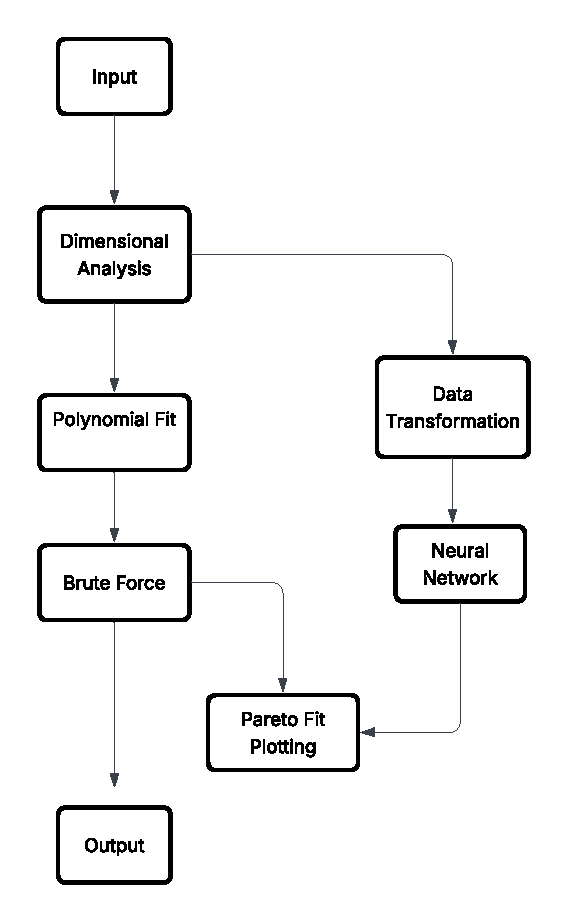
\includegraphics[width=7cm]{SR_Flow}
    \caption{The SR control flow for the solver, show in this diagram above.} % Optional
    \label{fig:sr_flow}
\end{figure}\\


\subsection{Testing:}
Every module, function and file, were thoroughly tested using dedicated tests. The boundary conditions and
inserted tests to make sure the function behaved as envisioned. There was also significant robust testing func-
tions written when chaining together various techniques and models, in order to ensure everything was working
smoothly.\\

\subsubsection{Unit Testing: }

I've written unit tests for every function, every evaluation method and have rigorously tested their functionality, edge cases, normal inputs etc. \\

Rigorous unit testing was employed to validate the correctness of each module within the symbolic regression framework. Key components including Pareto frontier operations, polynomial generation and evaluation, and dimensional analysis routines were individually tested using structured unit tests. Each test assessed expected outputs under standard and edge-case inputs.

Test results confirmed correct behavior, and outputs aligned with theoretical expectations (e.g., correct Pareto set retrieval, successful polynomial fitting on synthetic data, and dimensionally consistent variable transformations). A summary of testing outcomes is shown below. Furthermore, synthetic datasets based on known biological formulas were used to validate the regressor’s ability to recover exact symbolic relationships, demonstrating the system’s practical reliability.\\



% Please add the following required packages to your document preamble:
% \usepackage{graphicx}
% \usepackage[table,xcdraw]{xcolor}
% Beamer presentation requires \usepackage{colortbl} instead of \usepackage[table,xcdraw]{xcolor}
\begin{table}[]
\resizebox{\columnwidth}{!}{%
\begin{tabular}{|l|l|l|}
\hline
\textit{\textbf{Module:}} & \textit{\textbf{Tests:}}                   & \textit{\textbf{Results:}}    \\ \hline
Dimensional Analysis & Get, Solve, Generate, Symbolic Transformation                                    & {\color[HTML]{000000} Passed} \\ \hline
Neural Network       & Load, Network, Train, Predict, Gradient                                          & {\color[HTML]{000000} Passed} \\ \hline
Plotting                  & Pareto, Gradient                           & {\color[HTML]{000000} Passed} \\ \hline
Polynomial Regressor      & Load, Generate, Filter, Evaluate, Best fit & Passed                        \\ \hline
Brute Force          & Load, Generate, Recursive, Evaluate, Loss, Variable Filtering, Constants, Powers & Passed                        \\ \hline
Main Solver               & Main Solver, Laws                          & Passed                        \\ \hline
\end{tabular}%
}
\end{table}\\



\subsubsection{Integration Testing: }

To validate the interoperability and functional correctness of the developed software system, a comprehensive suite of integration tests was designed and executed. These tests focused on the interactions between the core Python modules, including Dimensional Analysis (dimensionalAnalysis), Polynomial Fitting (polynomialFit), Brute-Force Symbolic Regression (bruteForce), Neural Network (neuralNetwork) components, Pareto front optimization (pareto), and visualization (plots). Utilizing Python's unittest framework, the tests simulated realistic data analysis workflows, verifying the seamless flow of data and control between modules. This chaining of multiple methods was partially inspired by \cite{cranmer2023}, showing that it is far more effective to employ this architecture when aiming to prune the search tree.\\

Some of the key tested interactions included the preprocessing of data using Dimensional Analysis feeding into various model fitting approaches (PF, BF, NN), the evaluation of candidate expressions generated by BF and PF modules and their subsequent management on a Pareto front, and the symbolic transformation capabilities of the Dimensional Analysis module. Further tests confirmed the internal consistency of complex operations within the Brute-Force module and the functionality of gradient calculations in the Neural Network. Successful execution of these tests demonstrates the robustness of the integrated system and its capability to perform complex, multi-stage symbolic regression tasks as designed, ensuring reliable data handoffs.\\



\subsubsection{Performance Testing: }


To quantitatively evaluate the computational efficiency and scalability of the core symbolic regression components, dedicated performance tests were executed on the bruteForce and polynomialFit modules. Utilizing Python scripts leveraging the time module for execution duration measurement and the psutil library for monitoring Resident Set Size (RSS) memory usage, these tests targeted the primary computational bottlenecks: symbolic expression generation and expression evaluation against numerical data.\\

The methodology involved systematically varying key parameters influencing complexity, such as expression generation depth (bruteForce), maximum polynomial degree (polynomial fit), the number of input variables, and the size of the input data sample for evaluation. By recording execution time and memory consumption under these varying conditions, the tests aimed to characterize the performance scaling of each module's algorithms. This analysis provides crucial insights into the computational complexity and resource requirements for each of the approaches, facilitating an understanding of their practical limitations and scalability characteristics. The results quantify the performance trade-offs inherent in different symbolic search strategies and inform the feasibility of applying the developed system to large-scale scientific discovery tasks by establishing empirical benchmarks for time and memory demands.\\





\section{ Applying the model to Biological Data: }




\subsubsection{Wallace Rule: }

While symbolic regression has demonstrated considerable success in modelling physical systems, its application to biological domains remains largely underexplored. Biological processes are inherently noisy, high-dimensional, and complex, often lacking explicit or well-defined governing equations. This complexity has contributed to a significant research gap in the application of symbolic regression techniques to biological data modelling \cite{willard2022}. Only a limited number of studies have pursued this direction, positioning it as a novel and potentially transformative area of research.\\

So applying it to biological data could be useful in helping speed up biological advancement, symbolic regression is applied to a fundamental biological phenomenon here: the prediction of nucleic acid melting temperature (Tm) from DNA/RNA base counts. The melting temperature is estimated using the Wallace rule, a well-established empirical relationship defined as follows:\\


\begin{equation}
    T_m = 2(A + T) + 4(G + C)
\end{equation}
where $A$, $T$, $G$, and $C$ represent the counts of adenine, thymine, guanine, and cytosine bases, respectively.\\


Evaluating the regression system, synthetic datasets were generated. Each sample point consists of four integer inputs representing each of the bases, and the corresponding target values are computed precisely using this formula. Variables (\texttt{['A', 'T', 'G', 'C']}) and constants (\texttt{[2, 4]}) are explicitly defined, and are passed into the regressor model.\\

The symbolic regression pipeline begins with dimensional analysis, although units in biological contexts are generally less rigorously defined than in physics. The system proceeds through a hybrid pipeline that includes polynomial fitting, and brute-force expression search. This multi-stage approach is designed to recover the underlying functional form governing the input-output relationship.\\

This shows the potential to find complex relationships between genes in a mathematical language we grasp better. \\



\section{Evaluation:}

To evaluate the two models, a Python script was executed to compare both memory usage and execution time. The results indicate that the custom model consumes significantly more memory and is slower by approximately an order of magnitude compared to PySR.\\

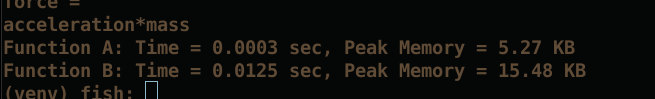
\includegraphics[width=10cm]{Eval_2}

Furthermore, the custom model lacks the accuracy and comprehensive search capabilities offered by PySR. While the custom implementation may identify the correct expression, PySR not only achieves this but also generates a variety of alternative approximations.\

Overall, PySR demonstrates greater versatility and robustness in symbolic regression tasks. Perhaps using genetic algorithms can help speed up the searches. \\
Genetic programming-based models, such as Eureqa, evolve expressions over time using operations inspired by biological evolution. These models are flexible and capable of discovering highly nonlinear relationships but often require significant computational resources and tuning. More recently, neural-symbolic models like AI Feynman and PySR have emerged, combining machine learning with symbolic manipulation. Also PINN's could've helped speed up the search space, and allow the program to discover more complex, non linear laws.\\ 





\end{document}
